%!TeX program=xelatex
\documentclass[a4paper]{article}

\usepackage{amsmath}
\usepackage{amssymb}
\usepackage[margin=1in]{geometry}
\usepackage{xcolor}
\usepackage{graphicx}
\usepackage{algorithm2e}
\usepackage{hyperref}
\hypersetup{
    colorlinks,
    linkcolor={red!50!black},
    citecolor={blue!50!black},
    urlcolor={green!50!black}
}
\usepackage{subcaption}
\usepackage[numbers]{natbib}
\usepackage[usenames,dvipsnames]{pstricks}
\usepackage{epsfig}
\usepackage{pgf}

\usepackage{fontspec}
\setmainfont[Ligatures=TeX]{Palatino Linotype}

\newcommand{\fig}{Figure }
\newcommand{\sect}{Section }
\newcommand{\app}{Appendix }

\begin{document}
  {\Large\noindent  Machine Learning on the Radio Galaxy Zoo}\\

  {\large\noindent  Matthew Alger \hfill Supervisor: Cheng Soon Ong}\\

  {\large\noindent  June 3, 2016}\\

  \begin{abstract}
    I did something and it kinda worked
  \end{abstract}

  \section{Introduction}

    \subsection{Cross-identification of Radio Sources and Host Galaxies}

      Radio surveys such as Faint Images of the Radio Sky at Twenty-Centimeters (FIRST) \cite{white97,becker95} and the Australian Telescope Large Area Survey (ATLAS) \cite{franzen15} have found many sources of radio emissions. These radio sources are dominated by \emph{active galactic nuclei} (AGNs) \cite{banfield15}, galactic centres with supermassive black holes that emit radio waves\cite{peterson97}. Galaxies containing a radio source are referred to as \emph{host galaxies}. These galaxies are found in infrared surveys such as the Wide-field Infrared Survey Explorer (WISE) \cite{wright10} and the SIRTF Wide-area Infrared Extragalactic survey (SWIRE) \cite{surace05,lonsdale03}.

      Astrophysicists are interested in the properties of both AGNs and their host galaxies, but to investigate either, the radio sources need to be matched to their host galaxies. This is called \emph{cross-identification}. Many radio sources are \emph{compact radio sources}, where the radio emissions directly and simply overlap the host galaxy (\fig \ref{fig:compact-source}). These radio sources are easy to cross-identify\cite{banfield15}. However, many radio sources are instead \emph{complex radio sources}, where radio emissions can be large, sprawling, and not relate to the host galaxy in any simple way (\fig \ref{fig:complex-source}).

      \begin{figure}[!ht]
        \centering
          \begin{subfigure}{0.3\textwidth}
            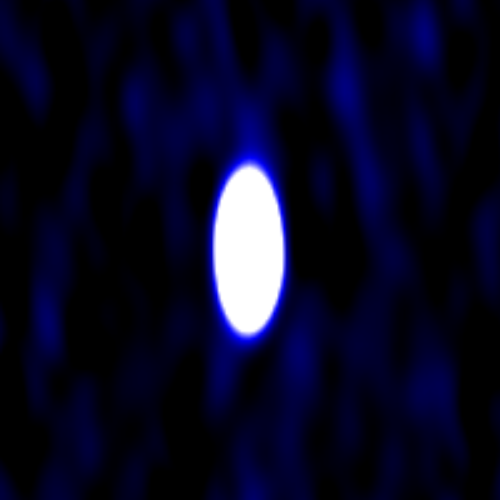
\includegraphics[width=\linewidth]{images/ARG0003r22_radio.png}
            \caption{A compact radio source.}
            \label{fig:compact-source}
          \end{subfigure}
          \quad
          \begin{subfigure}{0.3\textwidth}
            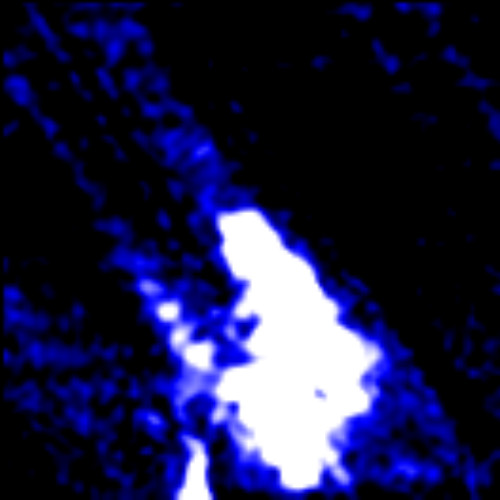
\includegraphics[width=\linewidth]{images/ARG0002dun_radio.jpg}
            \caption{A complex radio source.}
            \label{fig:complex-source}
          \end{subfigure}
          \caption{Example radio emissions.}
      \end{figure}

      \emph{Radio Galaxy Zoo}\footnote{\href{http://radio.galaxyzoo.org/}{Radio Galaxy Zoo}} is an online citizen science project that aims to crowdsource the cross-identification problem\cite{banfield15}. Volunteers are presented with a radio image of a small part of the sky (from FIRST or ATLAS) and the corresponding infrared image (from WISE or SWIRE). Each part of the sky presented in this way is called a \emph{subject}, and contains at least one radio emitter. Volunteers are asked to select which radio emissions are part of the same system, and which galaxy in the infrared image contains the corresponding AGN. The workflow is shown in \fig \ref{fig:rgz}.

      \begin{figure}[!ht]
        \centering
          \begin{subfigure}{0.3\textwidth}
            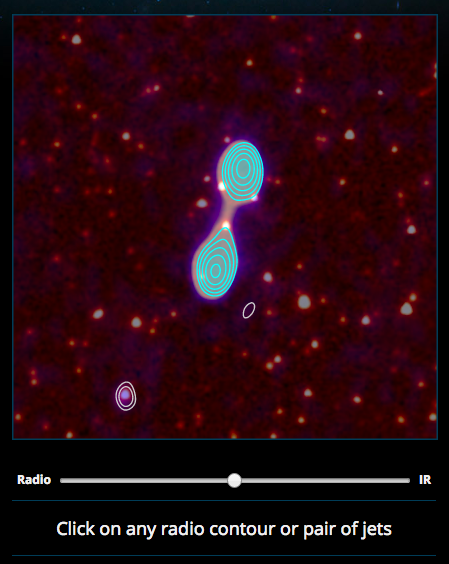
\includegraphics[width=\linewidth, height=2.3in]{images/rgz_radio.png}
            \caption{Select radio emissions.}
          \end{subfigure}
          \quad
          \begin{subfigure}{0.3\textwidth}
            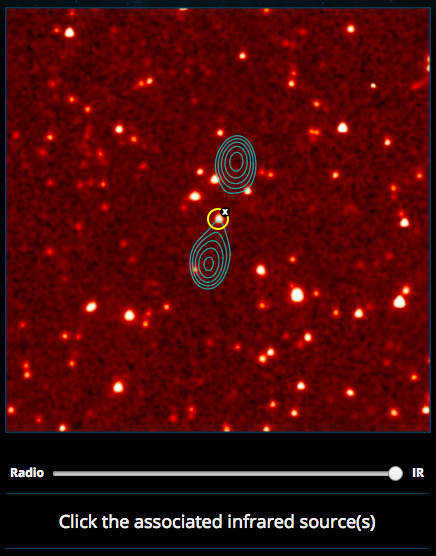
\includegraphics[width=\linewidth, height=2.3in]{images/rgz_ir.png}
            \caption{Locate the AGN.}
          \end{subfigure}
          \quad
          \begin{subfigure}{0.3\textwidth}
            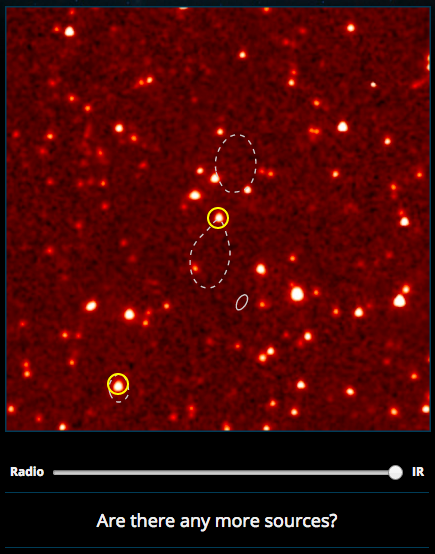
\includegraphics[width=\linewidth, height=2.3in]{images/rgz_done.png}
            \caption{Repeat for all emissions.}
          \end{subfigure}
          \caption{Radio Galaxy Zoo volunteer workflow.}
          \label{fig:rgz}
      \end{figure}

      To increase cross-identification accuracy, each compact radio source is presented to $5$ volunteers, and each complex radio source is presented to $20$ volunteers\cite{banfield15}.

      Over 100 000 radio sources have been cross-identified by volunteers so far\footnote{Based on the data supplied to the author.} out of the Radio Galaxy Zoo database of around 177 000 radio sources, compared to a few thousand classifications by experts\cite{banfield15}. However, new surveys such as the Evolutionary Map of the Universe (EMU) \cite{norris11} and Westerbork Observations of the Deep APERTIF Northern-Sky (WODAN) \cite{röttgering11} are expected to detect over 100 million radio sources\cite{banfield15}, making crowdsourcing an intractable solution to the cross-identification problem.

      In this report, I describe my research into using cross-identifications made by Radio Galaxy Zoo volunteers as a training set for training supervised machine learning algorithms to automatically perform the cross-identification task.

    \subsection{Related Work}

      Proctor 2006\cite{proctor06}; Kimball \& Ivezić 2008; van Velzen, Falcke, \& Körding 2015

      \citet{fan15} developed an probabilistic, automated method of cross-identifying radio sources and host galaxies based on explicit radio source models. They modelled radio sources as a central radio object and two surrounding lobes in an approximately straight line, as would be expected of emissions from a black hole. They achieved $85.8\%$ cross-identification accuracy against the manual cross-identifications made by \citet{norris06}. While their method is limited by its dependence on the model, it is also easily extended to different models, and so may provide a good basis for future astronomical model-based work. Their method is also able to determine whether nearby radio objects are part of the same source. This is one of the problems Radio Galaxy Zoo is attempting to solve, as collating radio objects is a difficult task for computers.

  \section{Data Sources}

    \subsection{ATLAS}

      ATLAS is a radio-wavelength survey of the Chandra Deep Field South (CDFS) and the European Large Area ISO Survey -- South 1 (ELAIS-S1) fields, which were chosen as they are both areas of the sky covered by the earlier SWIRE survey. This means that the ATLAS observations have corresponding observations in infrared wavelengths\cite{franzen15}. Infrared observations are necessary for cross-identification, since the distant galaxies we want to cross-identify the radio objects with emit infrared radiation.

      While the Radio Galaxy Zoo data include classifications of objects in both the ATLAS and FIRST surveys, here I have only focused on the ATLAS observations of CDFS. Firstly, ATLAS contains only 2400 objects. This is a good size --- large enough to train supervised machine learning models, but small enough to quickly iterate on these models as is required for such exploratory research. Secondly, ATLAS is mostly well-behaved, compact objects. While the eventual goal of this project is to be able to automatically cross-identify even very complicated complex sources, being able to accurately cross-identify simple compact sources is a necessary step. Thirdly, ATLAS is considered a ``test run'' for the much larger EMU survey, as EMU is similar in resolution to ATLAS\cite{franzen15}. EMU is where many new radio observations will be made, and the scale of the survey is a key motivator behind this project. Finally, ATLAS subjects have been cross-identified by experts already\cite{norris06}, meaning that I do not need to rely entirely on volunteer consensuses from the crowdsourced Radio Galaxy Zoo, and I can thus better validate and evaluate my results.

      ATLAS observations of CDFS consist of a $3.6 \text{ deg}^2$ mosaic of radio images between $3^\text{h}26^\text{m} 27^\circ 00'$ and $3^\text{h}36^\text{m} 29^\circ 00'$. The full ATLAS image of the CDFS field is shown in \fig \ref{fig:cdfs}.

      \begin{figure}[!ht]
        \centering
        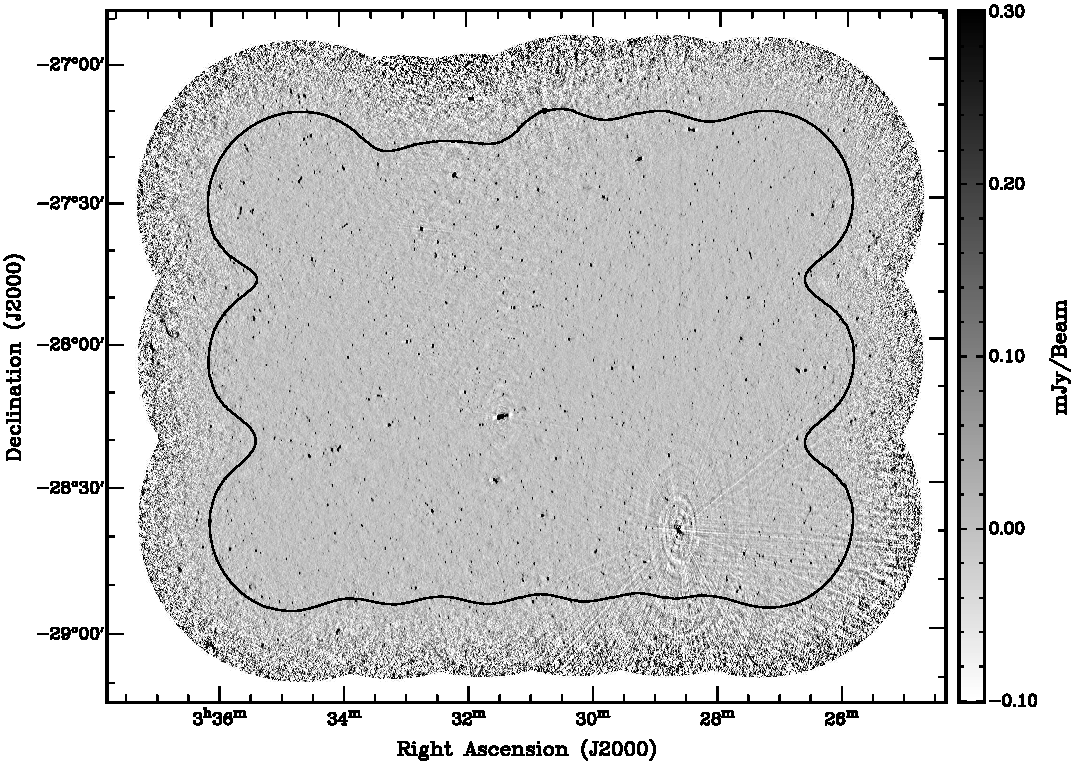
\includegraphics[width=0.8\linewidth,]{images/ATLAS-CDFS-cropped.pdf}
        \caption{ATLAS observations of CDFS. Reproduced from \citet{franzen15}.}.
        \label{fig:cdfs}
      \end{figure}

      Each ATLAS object forms a subject. Each subject consists of a $2' \times 2'$ image patch from \fig \ref{fig:cdfs} and a corresponding image patch from SWIRE centred on the associated ATLAS object.

    \subsection{SWIRE}

      SWIRE is an infrared-wavelength survey of seven regions of the sky in seven infrared bands. Of these regions, CDFS and ELAIS-S1 overlap with ATLAS and are hence used in Radio Galaxy Zoo.

      SWIRE observations are infrared images in the various fields, and are provided in Radio Galaxy Zoo as $2' \times 2'$ image patches centred on ATLAS subjects. In addition, I make use of the SWIRE CDFS Region Fall '05 Spitzer Catalog\cite{surace05}, which describes all objects detected in the CDFS field in the SWIRE survey.

      For each object in CDFS, the catalogue provides the name, location, infrared fluxes, and stellarity index associated with that object. The location is specified in right ascension and declination. The fluxes are given in five bands ($3.6\ \mu$Jy, $4.5\ \mu$Jy, $5.8\ \mu$Jy, $8.0\ \mu$Jy, and $24\ \mu$Jy) and describe how bright each object is in the corresponding flux band. Finally, the stellarity index is an indicator of how star-like each object is according to the SExtractor software package, where $0$ denotes an object that is totally non-star-like, and $1$ denotes an object that is totally star-like\cite{surace05}.

    \subsection{Radio Galaxy Zoo}

      Each ATLAS subject in the Radio Galaxy Zoo data is associated with a set of \emph{crowd classifications}, cross-identifications performed by volunteers. Each classification describes which radio objects near the subject the volunteer believes are part of the same radio source (called a \emph{radio combination}), as well as the location that the volunteer believes the corresponding host galaxy is located at.

      There are multiple classifications for each subject ($5$ for compact sources and $20$ for complex sources) to attempt to improve accuracy. These classifications differ from each other, so they need to be brought together in some way to identify a single radio combination/galaxy location label for each radio source in the data. The collated radio combinations for subjects are called \emph{radio consensuses}, the collated locations for a subject are called \emph{location consensuses}, and collated classifications on the whole are called \emph{consensuses}. Ideally, we want to take some ``majority vote'' and choose the most common radio combination as the radio consensus and then the most common corresponding locations as the location consensuses. The former is simple --- we just count the different combinations of radio objects and choose the most common --- but finding the location consensus is considerably more difficult as many different locations could represent the same host galaxy. \citet{banfield15} solve this problem by performing kernel density estimation on the locations associated with each radio combination, then choosing the location with the highest density. For this report, I have used a different method that uses a clustering algorithm called PG-means\cite{hamerly07}. The different locations are assigned to clusters, and the mean of the largest cluster becomes the location consensus.%, described later in \sect \ref{sec:consensuses}.

  \section{The Cross-identification Task}

    \subsection{Cross-identification as Binary Classification}

      The first step in applying machine learning methods to the cross-identification task is to find a machine learning framework that it fits in. The cross-identification task can be modelled as binary classification, allowing the use of standard binary classification methods. This is done as follows. For an ATLAS subject, consider all SWIRE objects within $1'$ Chebyshev distance of the corresponding ATLAS object's location, i.e., all galaxies that a volunteer would be allowed to choose from in the crowdsourced cross-identification task. These objects are called \emph{candidate hosts}. Each candidate is then either the host galaxy or not the host galaxy. ``Host galaxy'' and ``not host galaxy'' can thus be interpreted as two distinct classes, forming a binary classification problem. After training a classifier on this task, we can find the host galaxy in a subject by using the classifier to predict the probabilities that each candidate is the host galaxy, and then simply choose the candidate with the highest probability of being the host galaxy.\\

      % Formally, consider a set of candidates $\mathcal X$. Each candidate $x_i \in \mathcal X$ has a true label $t_i \in \{0, 1\}$, where $t_i$ is $1$ if $x_i$ is the host galaxy and $0$ otherwise. We want to select the candidate that maximises $p(t_i = 1 \mid x_i)$.

      % Formally, consider a set of candidates $\mathcal X$ and a function $t : \mathcal X \to \{0, 1\}$, defined such that $t(x)$ is $1$ if $x$ is the host galaxy and is $0$ otherwise. We want to find the $x \in \mathcal X$ that maximises the probability of $x$ being the host galaxy $p(t(x) = 1 \mid x)$:
      % Formally, we consider a set of candidates $\mathcal X$ and a set of labels $\mathcal Y = \{0, 1\}$. We want to find a function $y : \mathcal X \to \mathcal Y$ such that for $x \in \mathcal X$, $y(x)$ is $1$ if $x$ is a host galaxy, and $0$ otherwise.

      Note that I am ignoring the problem of having multiple host galaxies in a subject, and am assuming that any subject contains exactly one host. This is an oversimplification as there are indeed subjects that contain multiple hosts, but there are very few in the ATLAS data and they greatly increase the difficulty of the problem.

      % To train a binary classifier on this problem, we need to have both inputs to classify and target labels to predict. For labels, I make use of the Radio Galaxy Zoo consensuses. Each candidate is labelled with a `$1$' or a `$0$', where `$1$' means that the candidate is a host galaxy and `$0$' means that the candidate is not a host galaxy. For each consensus location in Radio Galaxy Zoo, the nearest SWIRE object is found and labelled `$1$'. All other objects are labelled `$0$'.

      % The inputs to the classifier are described in \sect \ref{sec:features}, and the labels are described in \sect \ref{sec:labels}.


    \subsection{Labels}
      \label{sec:labels}

      For training and evaluating the classifier, each SWIRE object is assigned a ``true'' label. This label comes from Radio Galaxy Zoo consensuses: For each consensus location found by Radio Galaxy Zoo volunteers, the nearest SWIRE object is labelled ``host galaxy''. All other SWIRE objects are labelled ``not host galaxy''.

      I make the assumption that these labels are accurate. However, this may not be the case, since volunteers may not correctly identify host galaxies. \citet{banfield15} found that when more than $75\%$ of volunteers agree, then their cross-identifications are as accurate as experts', and volunteers agree to this level on the vast majority of ATLAS subjects, so this assumption generally holds for the ATLAS Radio Galaxy Zoo classifications. It may not hold for other data sets such as the FIRST Radio Galaxy Zoo classifications.
      % \subsubsection{Collating Classifications}
      % \label{sec:consensuses}

      %   talk about pg means

    \subsection{Feature-space Representation of SWIRE Objects}
    \label{sec:features}

      To be able to classify a candidate, a feature-space representation of the candidate must be found. For a given candidate, the features used are to represent it are:
      \begin{itemize}
         \item the $3.6\ \mu$Jy flux of the candidate,
         \item the $4.5\ \mu$Jy flux of the candidate,
         \item the $5.8\ \mu$Jy flux of the candidate,
         \item the $8.0\ \mu$Jy flux of the candidate,
         \item the $24\ \mu$Jy flux of the candidate,
         \item the Chebyshev distance from the candidate to the nearest ATLAS object, and
         \item features extracted from patches of radio image centred on the candidate.
       \end{itemize}

      The infrared images around each candidate seem to contain little predictive information, and so are not included in the features.

      The radio patches are $0.8' \times 0.8'$ ($80\text{ px} \times 80\text{ px}$) images centred on each candidate. Features are extracted from these patches by a convolutional neural network. The network architecture is shown in \fig \ref{fig:cnn}. The network is pre-trained by appending a $32 \times 64$ dense layer and a $64 \times 1$ dense layer, then training the new convolutional neural network to find a map from the radio patches to the associated binary labels using backpropagation.

      \begin{figure}
        \centering
        % \usepackage[usenames,dvipsnames]{pstricks}
% \usepackage{epsfig}
% \usepackage{pst-grad} % For gradients
% \usepackage{pst-plot} % For axes
% User Packages:
% 
% 
\psscalebox{0.6 0.6} % Change this value to rescale the drawing.
{
\begin{pspicture}(0,-2.5333333)(20.966753,2.5333333)
\psframe[linecolor=black, linewidth=0.04, fillstyle=solid, dimen=outer](6.623895,1.8666667)(4.5667524,-0.1904762)
\psframe[linecolor=black, linewidth=0.04, fillstyle=solid, dimen=outer](7.1381807,1.352381)(5.081038,-0.7047619)
\psframe[linecolor=black, linewidth=0.04, fillstyle=solid, dimen=outer](7.652467,0.83809525)(5.5953236,-1.2190477)
\psframe[linecolor=black, linewidth=0.04, fillstyle=solid, dimen=outer](8.166752,0.32380953)(6.1096096,-1.7333333)
\psframe[linecolor=black, linewidth=0.04, fillstyle=solid, dimen=outer](11.242077,1.4666667)(9.766752,-0.008658009)
\psframe[linecolor=black, linewidth=0.04, fillstyle=solid, dimen=outer](11.6109085,1.0978355)(10.135584,-0.37748918)
\psframe[linecolor=black, linewidth=0.04, fillstyle=solid, dimen=outer](11.979739,0.7290043)(10.504415,-0.74632037)
\psframe[linecolor=black, linewidth=0.04, fillstyle=solid, dimen=outer](12.348571,0.36017317)(10.873246,-1.1151515)
\psframe[linecolor=black, linewidth=0.04, fillstyle=solid, dimen=outer](15.184934,1.0666667)(14.166752,0.048484847)
\psframe[linecolor=black, linewidth=0.04, fillstyle=solid, dimen=outer](15.43948,0.8121212)(14.421298,-0.2060606)
\psframe[linecolor=black, linewidth=0.04, fillstyle=solid, dimen=outer](15.694025,0.55757576)(14.675843,-0.46060607)
\psframe[linecolor=black, linewidth=0.04, fillstyle=solid, dimen=outer](15.94857,0.3030303)(14.930388,-0.7151515)
\psframe[linecolor=black, linewidth=0.04, fillstyle=solid, dimen=outer](18.203115,0.6666667)(17.766752,0.23030303)
\psframe[linecolor=black, linewidth=0.04, fillstyle=solid, dimen=outer](18.312206,0.55757576)(17.875843,0.121212125)
\psframe[linecolor=black, linewidth=0.04, fillstyle=solid, dimen=outer](18.421297,0.44848484)(17.984934,0.012121212)
\psframe[linecolor=black, linewidth=0.04, fillstyle=solid, dimen=outer](18.530388,0.33939394)(18.094025,-0.096969694)
\rput[bl](5.7667522,2.2666667){$32 \times 71 \times 71$}
\rput[bl](10.166752,2.2666667){$32 \times 14 \times 14$}
\rput[bl](14.166752,2.2666667){$32 \times 5 \times 5$}
\rput[bl](17.366753,2.2666667){$32 \times 1 \times 1$}
\psframe[linecolor=black, linewidth=0.04, dimen=outer](20.966753,1.0666667)(20.566751,-0.53333336)
\rput[bl](20.566751,2.2666667){$32$}
\psframe[linecolor=black, linewidth=0.02, fillstyle=solid, dimen=outer](8.051859,-0.8992908)(7.511433,-1.4397163)
\psframe[linecolor=black, linewidth=0.02, fillstyle=solid, dimen=outer](12.251859,0.10070922)(11.911433,-0.2397163)
\psframe[linecolor=black, linewidth=0.02, fillstyle=solid, dimen=outer](15.851859,-0.39929077)(15.711433,-0.5397163)
\psframe[linecolor=black, linewidth=0.02, fillstyle=solid, dimen=outer](12.151858,-0.69929075)(12.011434,-0.8397163)
\psframe[linecolor=black, linewidth=0.02, fillstyle=solid, dimen=outer](15.751859,0.0)(15.711433,-0.03971631)
\psframe[linecolor=black, linewidth=0.02, fillstyle=solid, dimen=outer](18.451859,0.10070922)(18.411432,0.060283687)
\psline[linecolor=black, linewidth=0.02](8.03614,-0.9071925)(12.03614,-0.7210884)
\psline[linecolor=black, linewidth=0.02](8.031646,-1.4239547)(12.040634,-0.825193)
\psline[linecolor=black, linewidth=0.02](12.23614,0.08831308)(15.7352915,-0.0063670413)
\psline[linecolor=black, linewidth=0.02](12.231646,-0.22844914)(15.726303,-0.028838951)
\psline[linecolor=black, linewidth=0.02](15.847376,-0.40831614)(18.434168,0.099250935)
\psline[linecolor=black, linewidth=0.02](15.847376,-0.5363143)(18.416191,0.06779026)
\psline[linecolor=black, linewidth=0.02](18.508915,0.31476077)(20.611092,1.0454048)
\psline[linecolor=black, linewidth=0.02](18.478146,-0.09016045)(20.58542,-0.5091328)
\psframe[linecolor=black, linewidth=0.04, fillstyle=solid, dimen=outer](2.6443307,1.3167521)(0.0,-1.3275784)
\rput[bl](0.8500857,2.2833333){$80 \times 80$}
\psframe[linecolor=black, linewidth=0.02, fillstyle=solid, dimen=outer](2.4299755,0.9778653)(1.7352916,0.28318152)
\psline[linecolor=black, linewidth=0.02](2.3764367,0.9770822)(7.6681905,0.008276656)
\psline[linecolor=black, linewidth=0.02](2.3706596,0.28333333)(7.6906343,-0.29167688)
\psframe[linecolor=black, linewidth=0.02, fillstyle=solid, dimen=outer](7.9685254,0.034042552)(7.6281,-0.30638298)
\rput[bl](12.000086,-2.4833333){$10 \times 10$
 convolution}
\rput[bl](16.050085,-2.5333333){$5 \times 5$
  max pooling}
\rput[bl](2.8000855,-2.4833333){$10 \times 10$
 convolution}
\rput[bl](8.050086,-2.5333333){$5 \times 5$
  max pooling}
\end{pspicture}
}


        \caption{Convolutional neural network for radio feature extraction. An $80 \times 80$ pixel patch of radio image (corresponding to $0.8' \times 0.8'$ of radio sky) is passed through two convolutional layers to obtain 32 features.}
        \label{fig:cnn}
      \end{figure}

      These features are all normalised, and the non-radio features are scaled. Scaling the radio features seems to significantly decrease classification accuracy, so I have chosen not to scale the radio features.

    \subsection{Classification Algorithm}
      \label{sec:algorithm}

      As input, we consider an ATLAS subject. We wish to automatically identify where the host galaxy that emitted this radio source is located. To perform this identification, we perform the following steps.

      \begin{enumerate}
        \item Identify all candidates (SWIRE objects) within $1'$ Chebyshev distance of the ATLAS subject.
        \item For each candidate, generate features (as described in \ref{sec:features}).
        \item Classify each candidate as being either the host galaxy or not being the host galaxy. This can be done with any classifier that can output a probability estimate.
        \item Select the candidate with the highest probability of being the host galaxy.
        \item Return the coordinates of the selected candidate.
      \end{enumerate}

      The above classification algorithm is pictured in \fig \ref{fig:pipeline}. In this report, I have experimented with using both logistic regression and random forest classifiers.

      \begin{figure}[!ht]
        \centering
        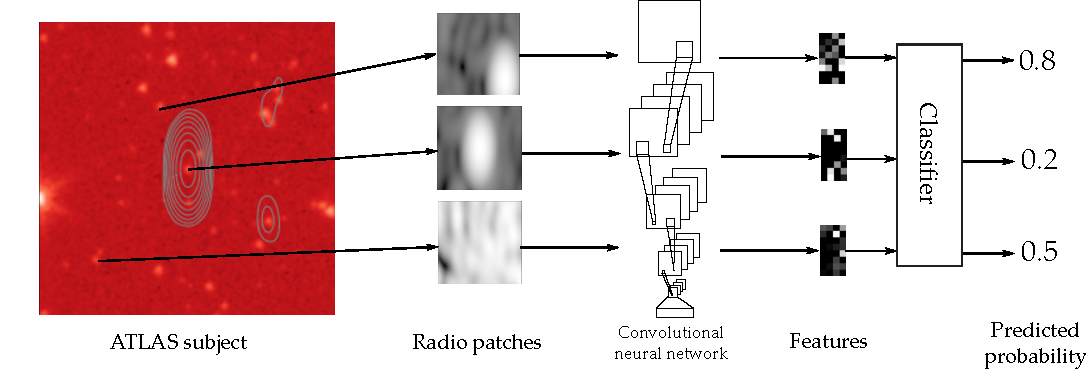
\includegraphics[width=0.9\linewidth]{images/pipeline.pdf}
        \caption{Classification algorithm. Non-image features are not pictured. Values are for indication only and are not the actual output of the classifier on the displayed inputs.}
        \label{fig:pipeline}
      \end{figure}

    \subsection{Evaluating the Classifier}

      There are two main ways to evaluate the classifier. Firstly, the classifier can be used to label a set of training SWIRE objects with known labels, and the classification accuracy can be found. This is very easy, but does not capture the cross-identification task --- labelling an individual SWIRE object may be more or less difficult than finding the host galaxy amongst a set of other candidate hosts. The second way to evaluate the classifier is to find the host coordinates for a set of training \emph{ATLAS subjects}, and then compare these coordinates to those found by Radio Galaxy Zoo volunteers. The performance measure is then how many ATLAS subjects the classifier is able to find the correct host location for.

  \section{Results}

    \subsection{Logistic Regression}

      Logistic regression was used in the classification algorithm described in \sect \ref{sec:algorithm}, with $1.0\ L_2$ regularisation. This resulted in $87.83\%$ classification accuracy when classifying individual SWIRE objects, and $72.12\%$ accuracy when finding the host galaxy for ATLAS subjects. The precision--recall and ROC curves for the individual classification task are displayed in \fig \ref{fig:precision-recall-roc-lr}, and the confusion matrix for the individual classification task is displayed in \fig \ref{fig:confusion-lr}. These metrics are not well-defined for the full host galaxy task, but sample outputs are displayed in \app I.

      \begin{figure}[!ht]
        \centering
        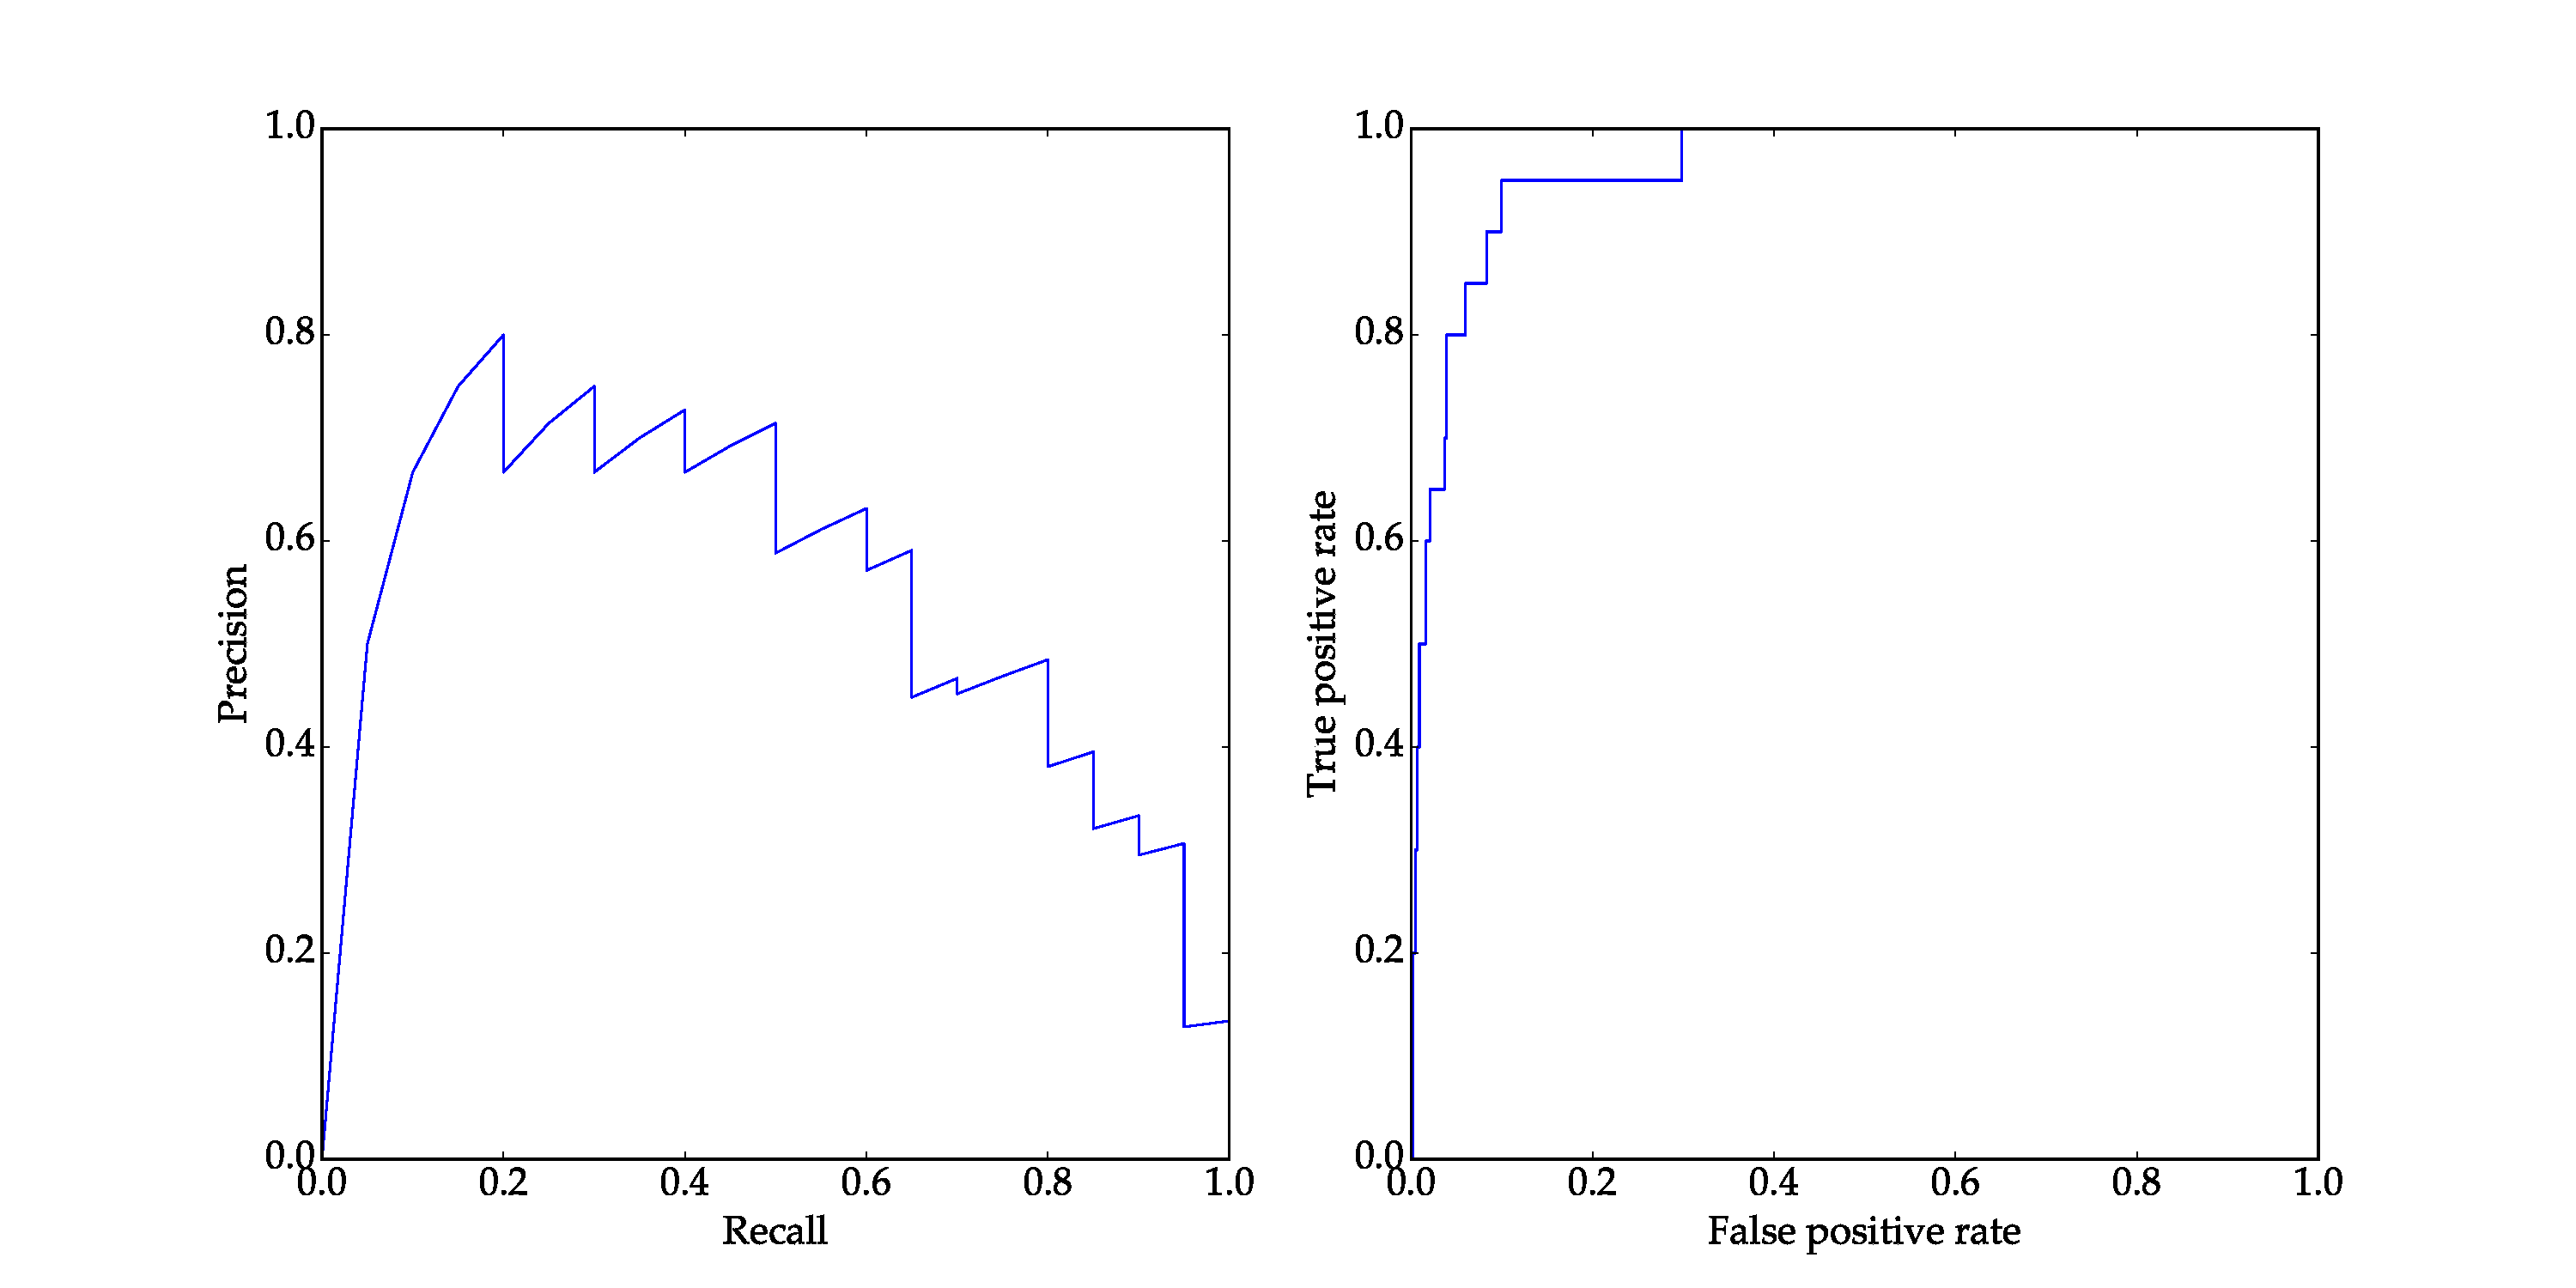
\includegraphics[width=\linewidth]{images/metrics_lr.pdf}
        \caption{Precision--recall and ROC curves for logistic regression on the individual SWIRE object classification task.}
        \label{fig:precision-recall-roc-lr}
      \end{figure}

      \begin{figure}[!ht]
        \centering
        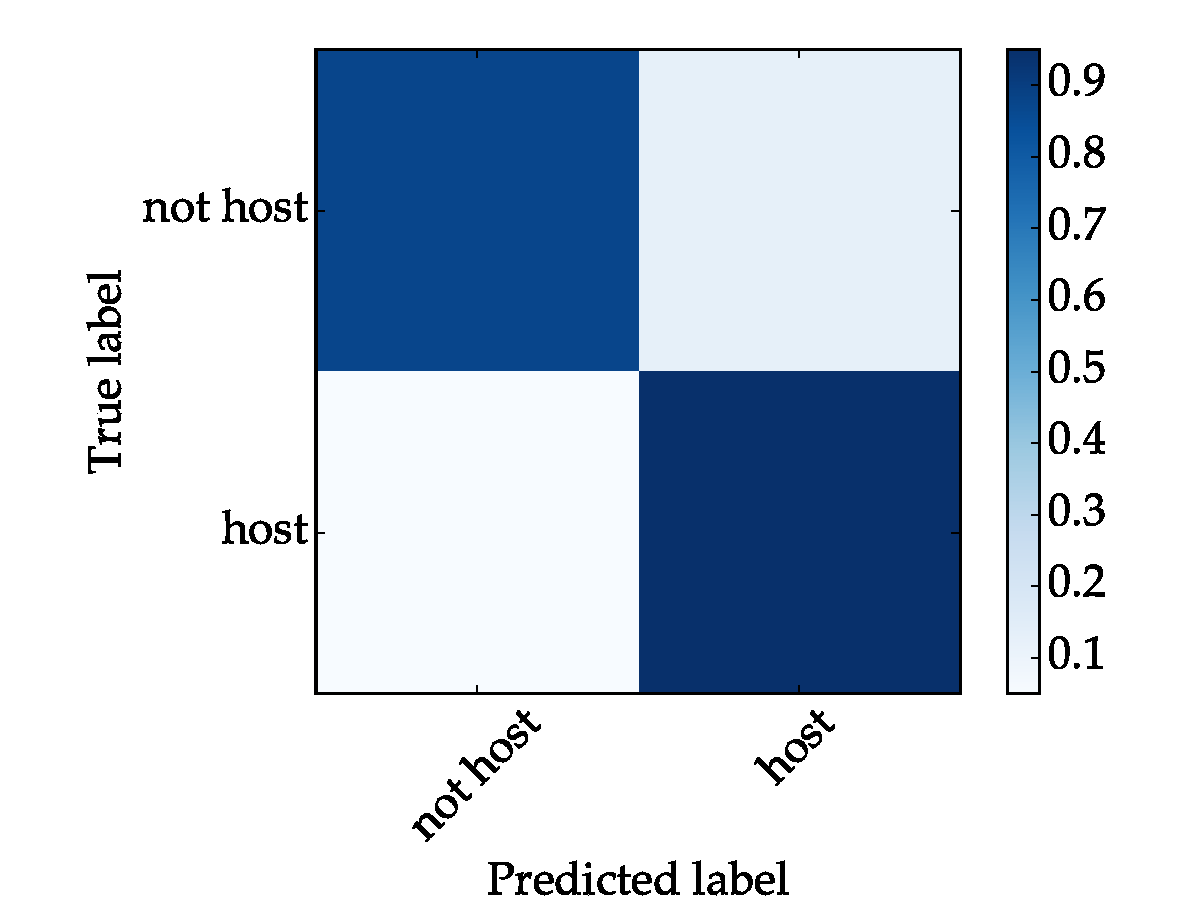
\includegraphics[width=0.5\linewidth]{images/confusion_lr.pdf}
        \caption{Confusion matrix for logistic regression on the individual SWIRE object classification task. The colour axis represents classification accuracy for each category.}
        \label{fig:confusion-lr}
      \end{figure}

    \subsection{Random Forests}

      Random forests with 10 trees were used in the classification algorithm described in \sect \ref{sec:algorithm}. This resulted in $99.34\%$ classification accuracy when classifying individual SWIRE objects, and $80.75\%$ accuracy when finding the host galaxy for ATLAS subjects. The precision--recall and ROC curves for the individual classification task are displayed in \fig \ref{fig:precision-recall-roc-rf}, and the confusion matrix for the individual classification task is displayed in \fig \ref{fig:confusion-rf}. These metrics are not well-defined for the full host galaxy task, but sample outputs are displayed in \app II.

      \begin{figure}
        \centering
        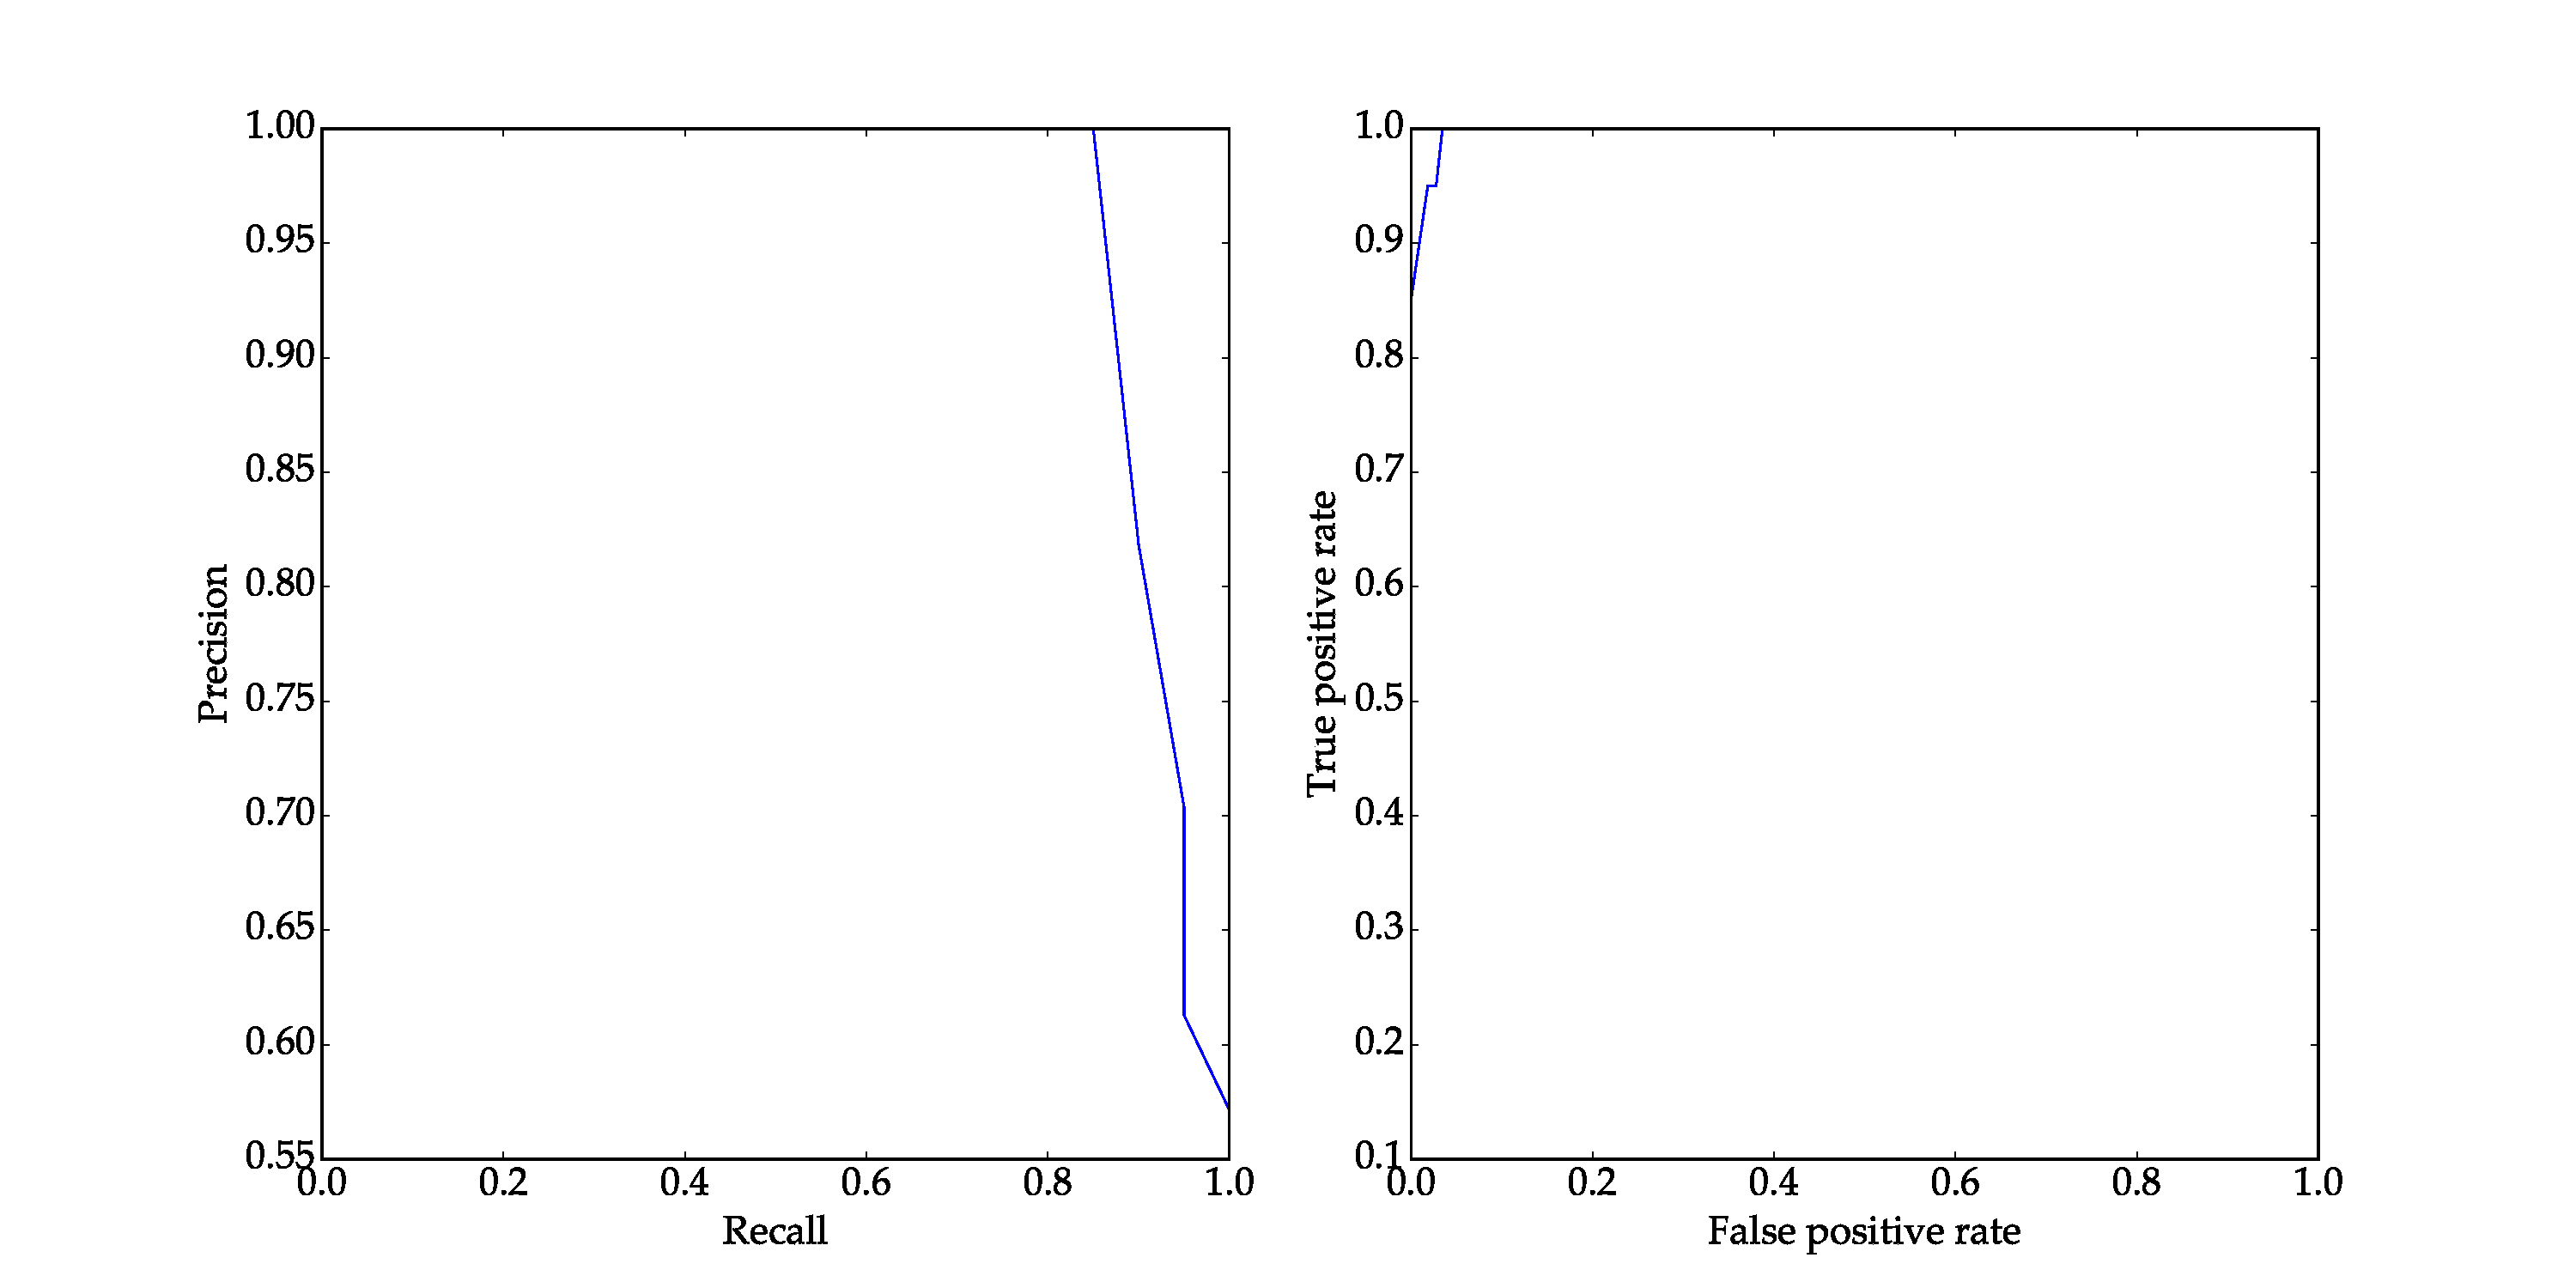
\includegraphics[width=\linewidth]{images/metrics_rf.pdf}
        \caption{Precision--recall and ROC curves for random forests on the individual SWIRE object classification task.}
        \label{fig:precision-recall-roc-rf}
      \end{figure}

      \begin{figure}
        \centering
        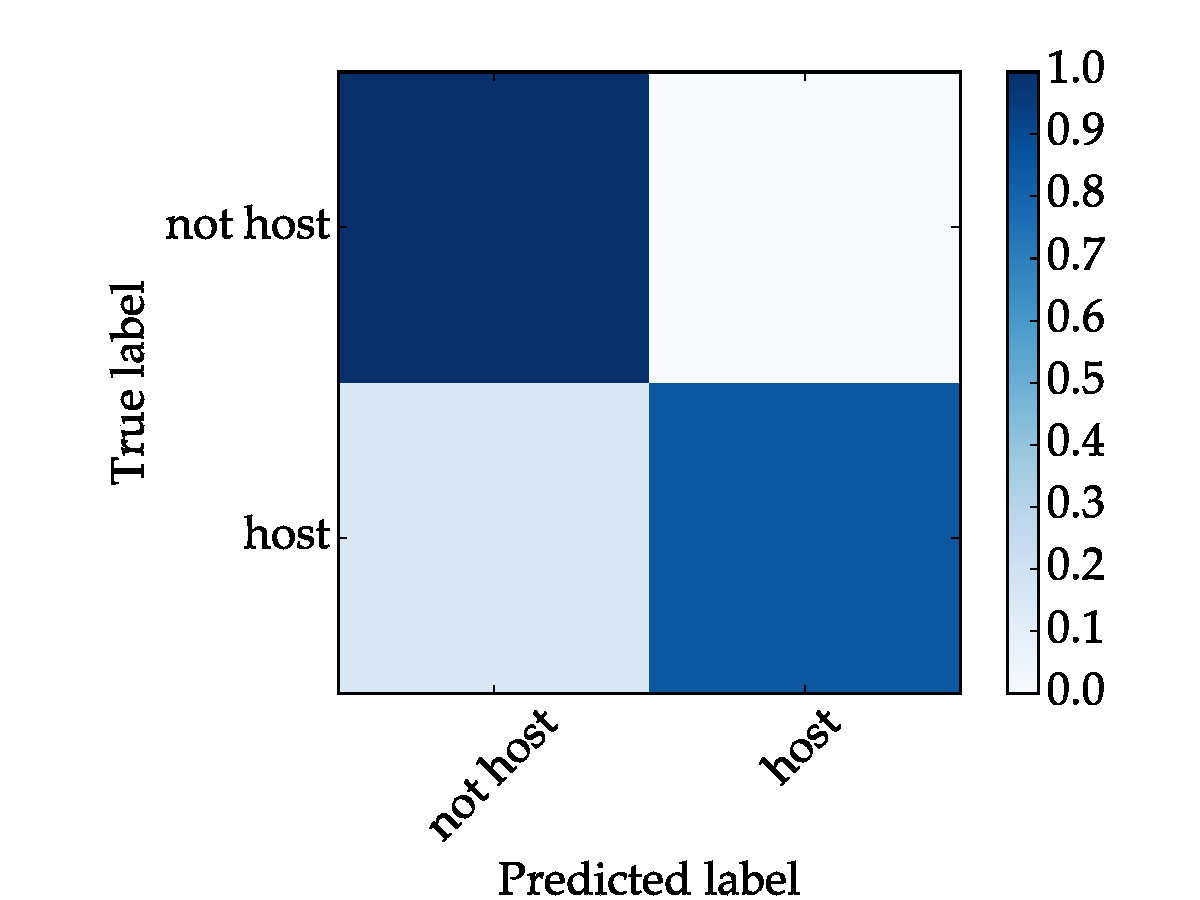
\includegraphics[width=0.5\linewidth]{images/confusion_rf.pdf}
        \caption{Confusion matrix for random forests on the individual SWIRE object classification task. The colour axis represents classification accuracy for each category.}
        \label{fig:confusion-rf}
      \end{figure}

    % show classification accuracies on the full problem, with and without different feature sets

  \section{Discussion}

  \section{Future Work}

    \begin{itemize}
      \item using the radio/location percentage consensuses to guess uncertainty
      \item model label noise
      \item active learning
    \end{itemize}

  \section{Conclusion}

  \bibliographystyle{abbrvnat}
  \bibliography{../papers}

  \newpage
  \section*{Appendix I}

    This appendix contains sample outputs from the logistic regression classifier. On the left of each figure is an ATLAS subject, with the infrared image from SWIRE in the background and intensity contours of the ATLAS radio image in the foreground. Candidate hosts are plotted on top of these images, coloured based on the predicted probability that they are the true host (where blue is least likely, and pink is most likely). On the right of each figure is a plot of each candidate's predicted probability with an arbitrary $x$ axis. The candidates have been sorted by increasing probability. This helps to visualise the spread of the probabilities.

    \begin{figure}[!ht]
      \centering
      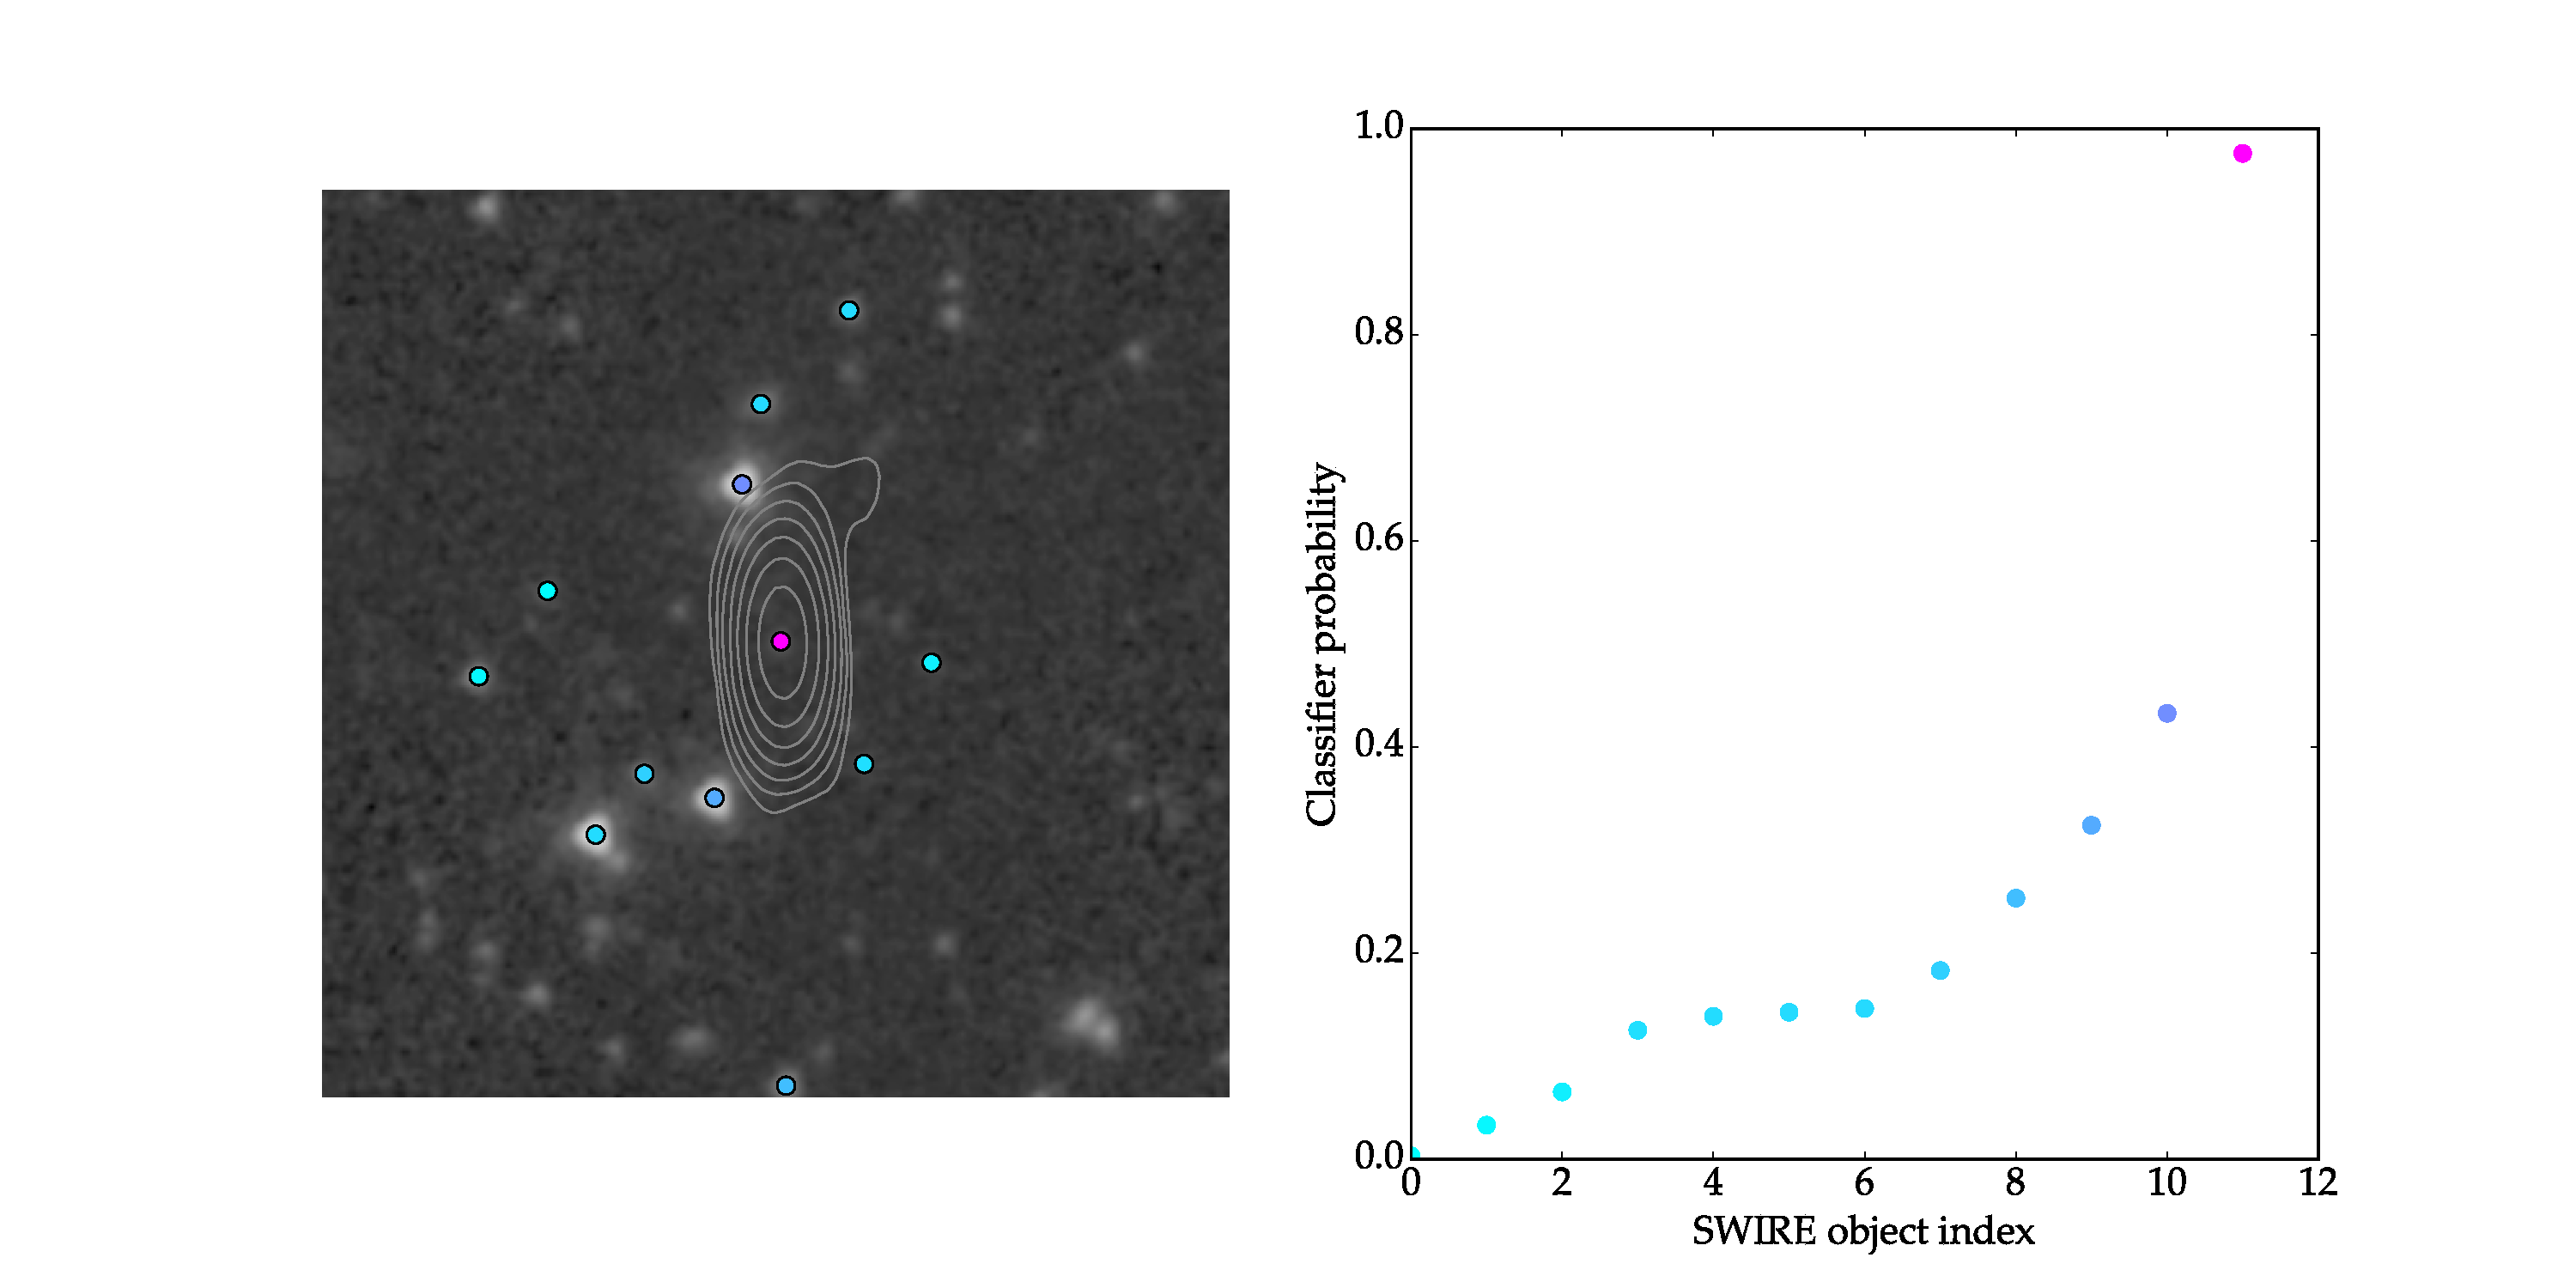
\includegraphics[width=\linewidth]{images/ARG0003r2o_lr.pdf}
      \caption{Logistic regression output for ARG0003r2o, an easy-to-classify compact source.}
      \label{fig:ARG0003r2o_lr}
    \end{figure}

    \begin{figure}[!ht]
      \centering
      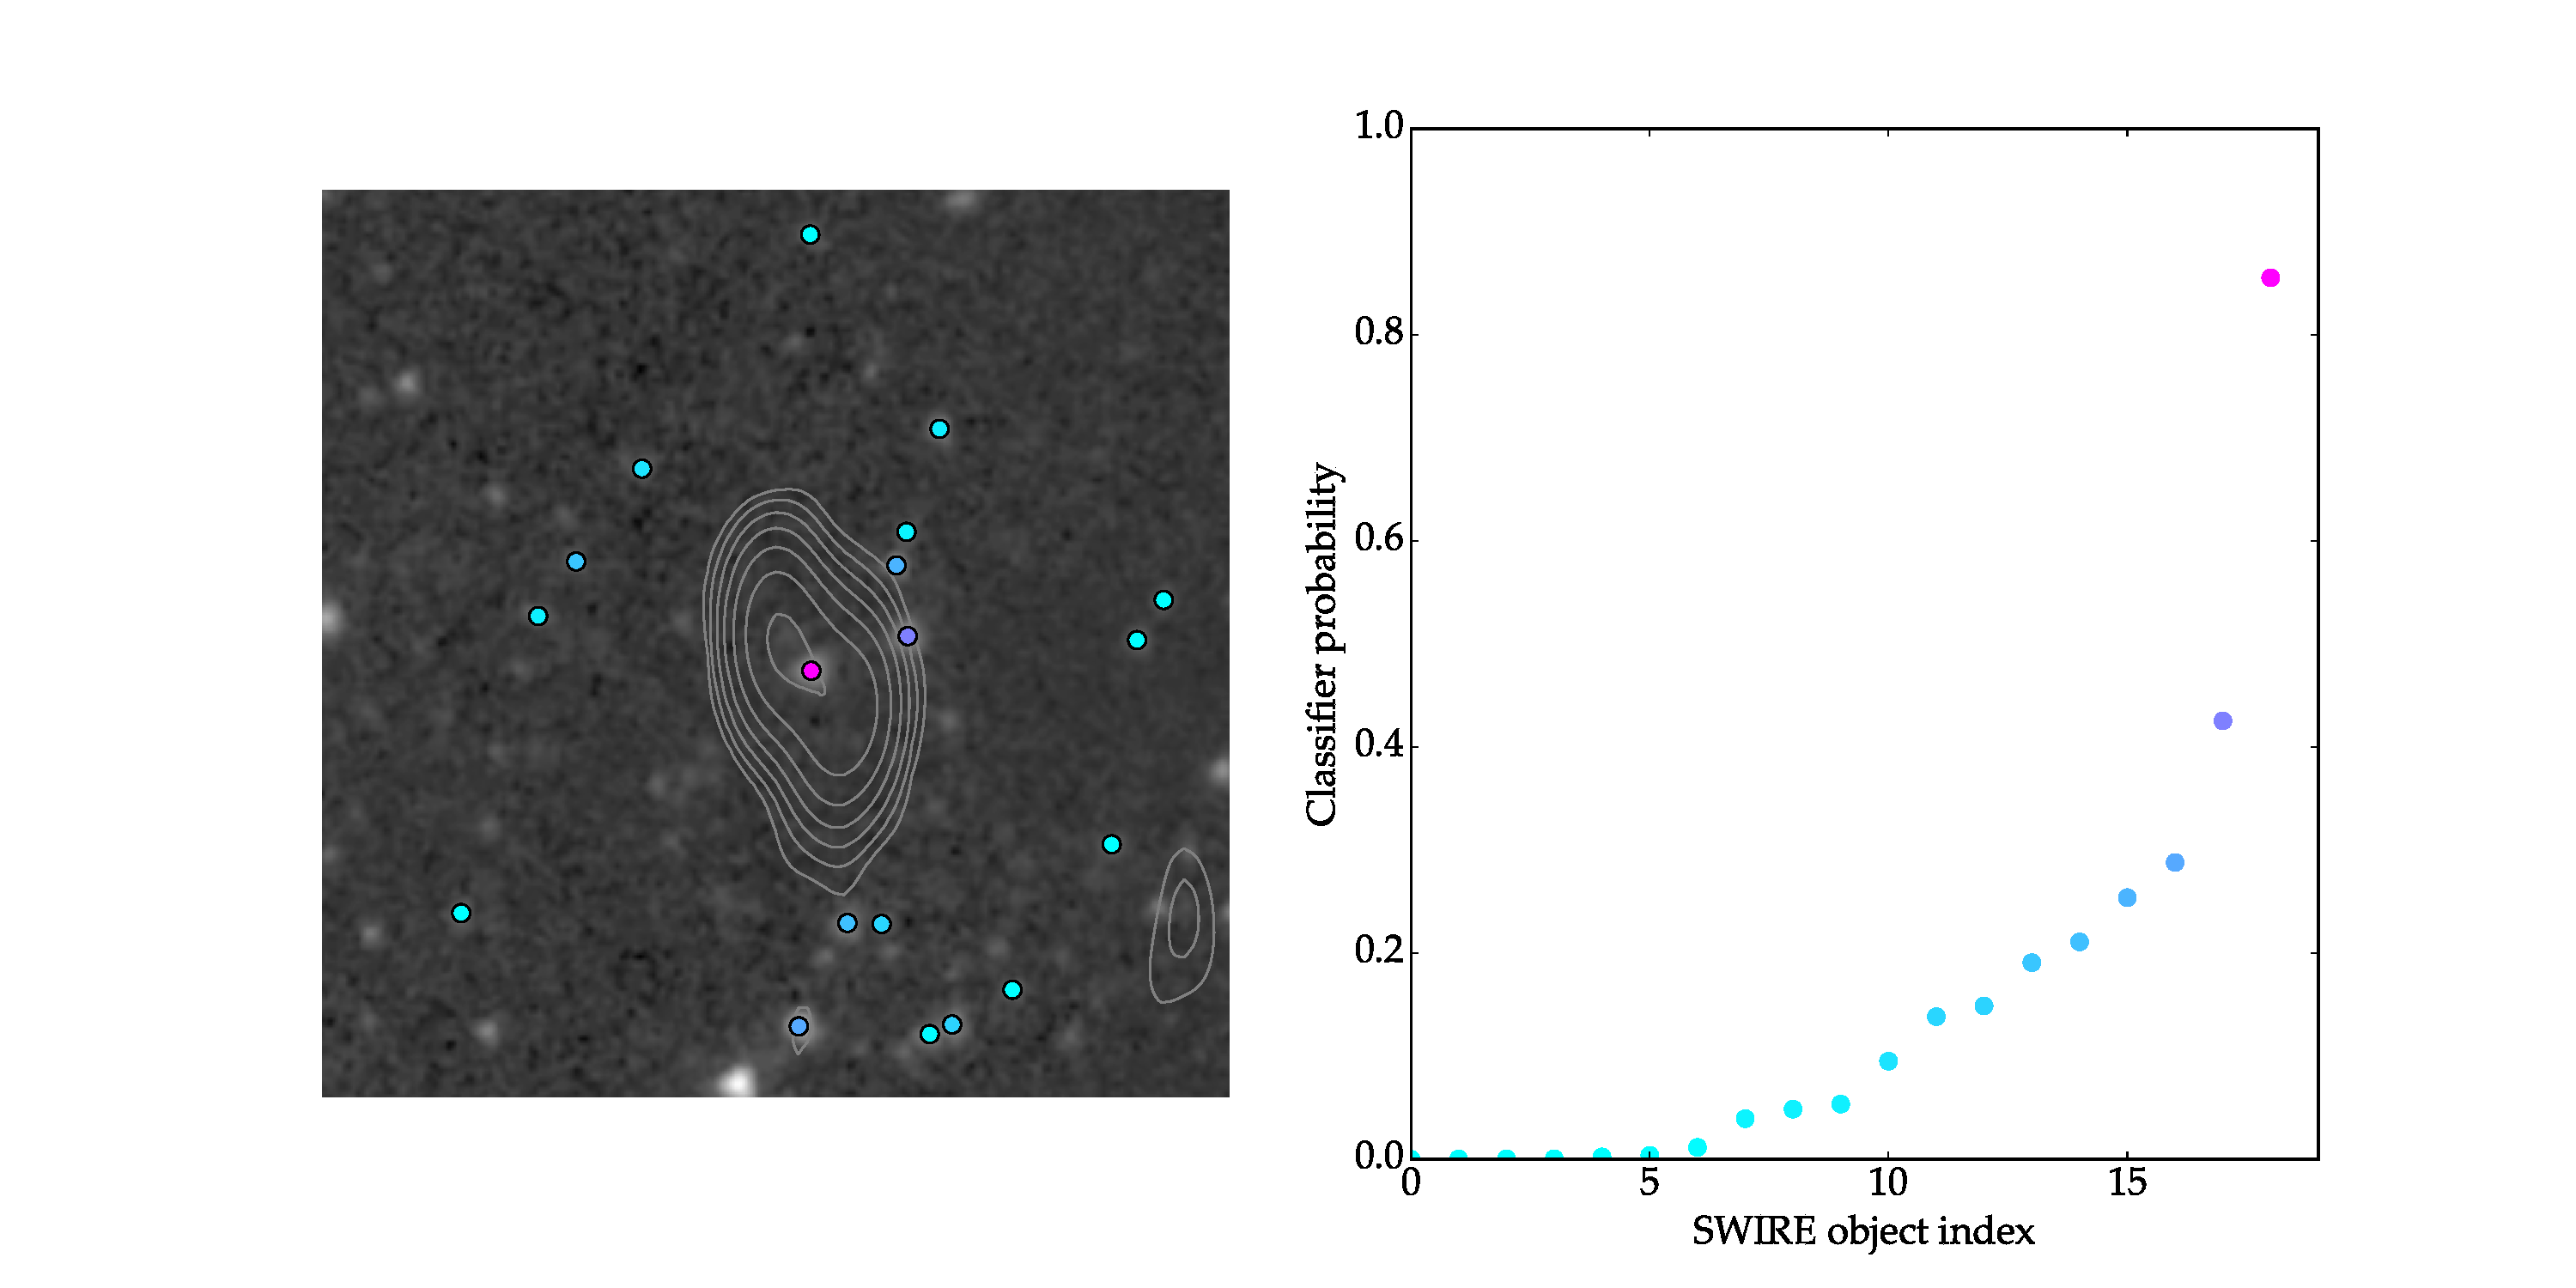
\includegraphics[width=\linewidth]{images/ARG0003r2w_lr.pdf}
      \caption{Logistic regression output for ARG0003r2w, an easy-to-classify compact source.}
      \label{fig:ARG0003r2w_lr}
    \end{figure}

    \begin{figure}[!ht]
      \centering
      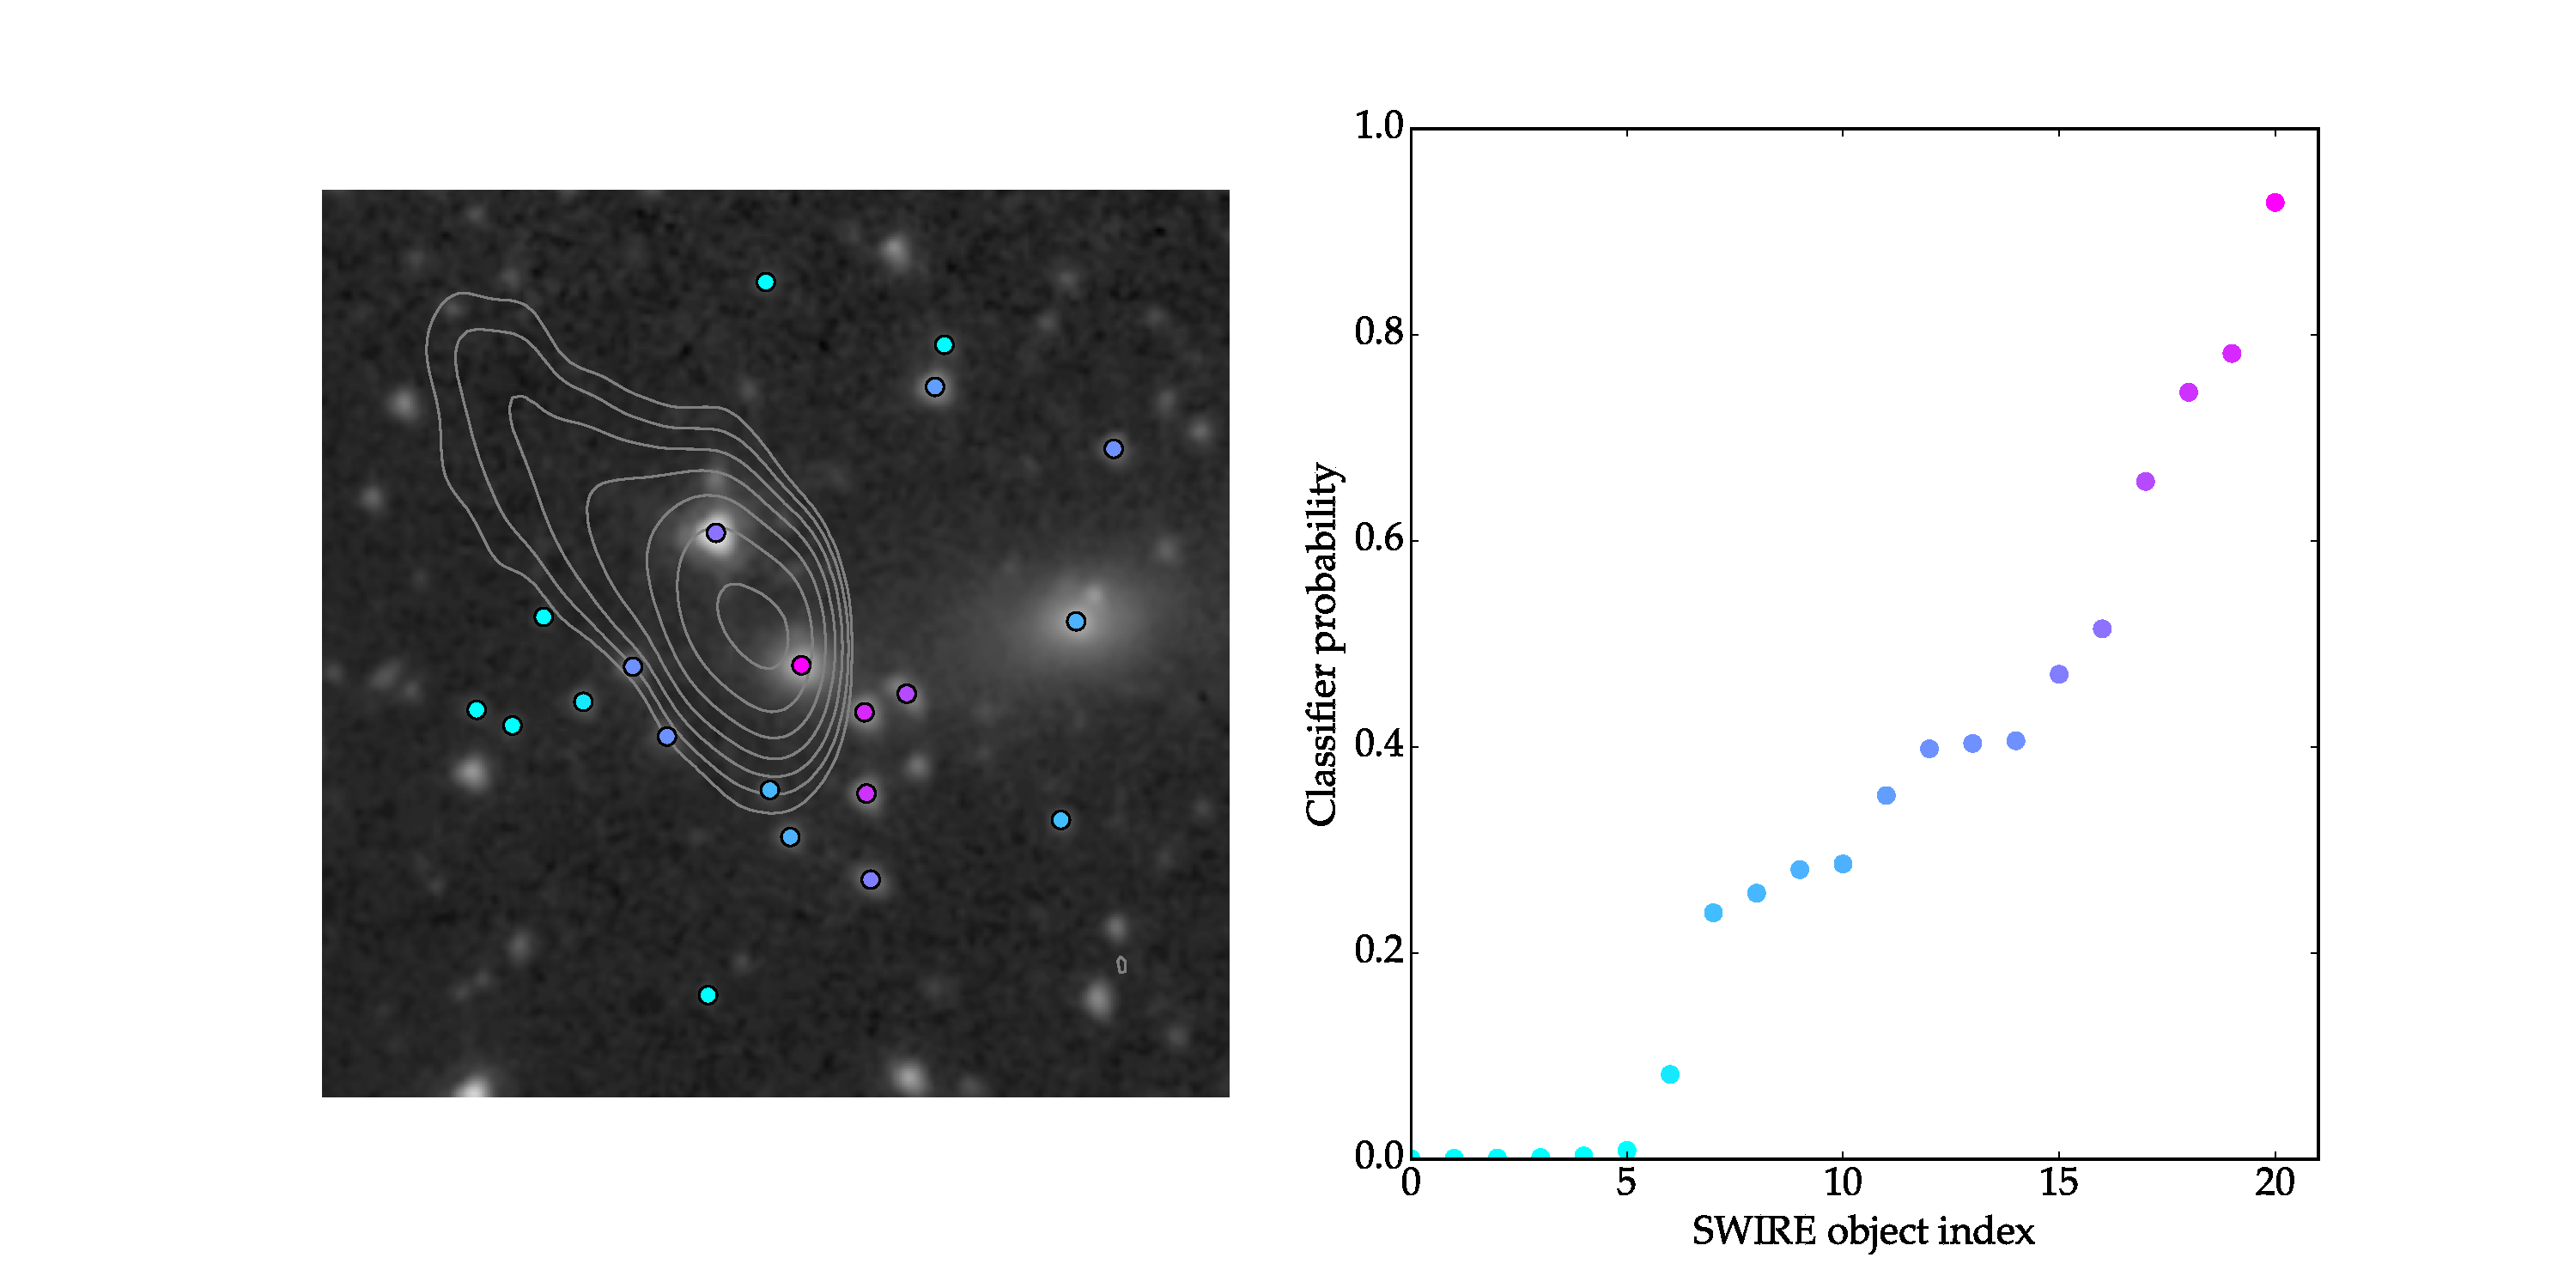
\includegraphics[width=\linewidth]{images/ARG0003r25_lr.pdf}
      \caption{Logistic regression output for ARG0003r25, a complex source.}
      \label{fig:ARG0003r25_lr}
    \end{figure}

    \begin{figure}[!ht]
      \centering
      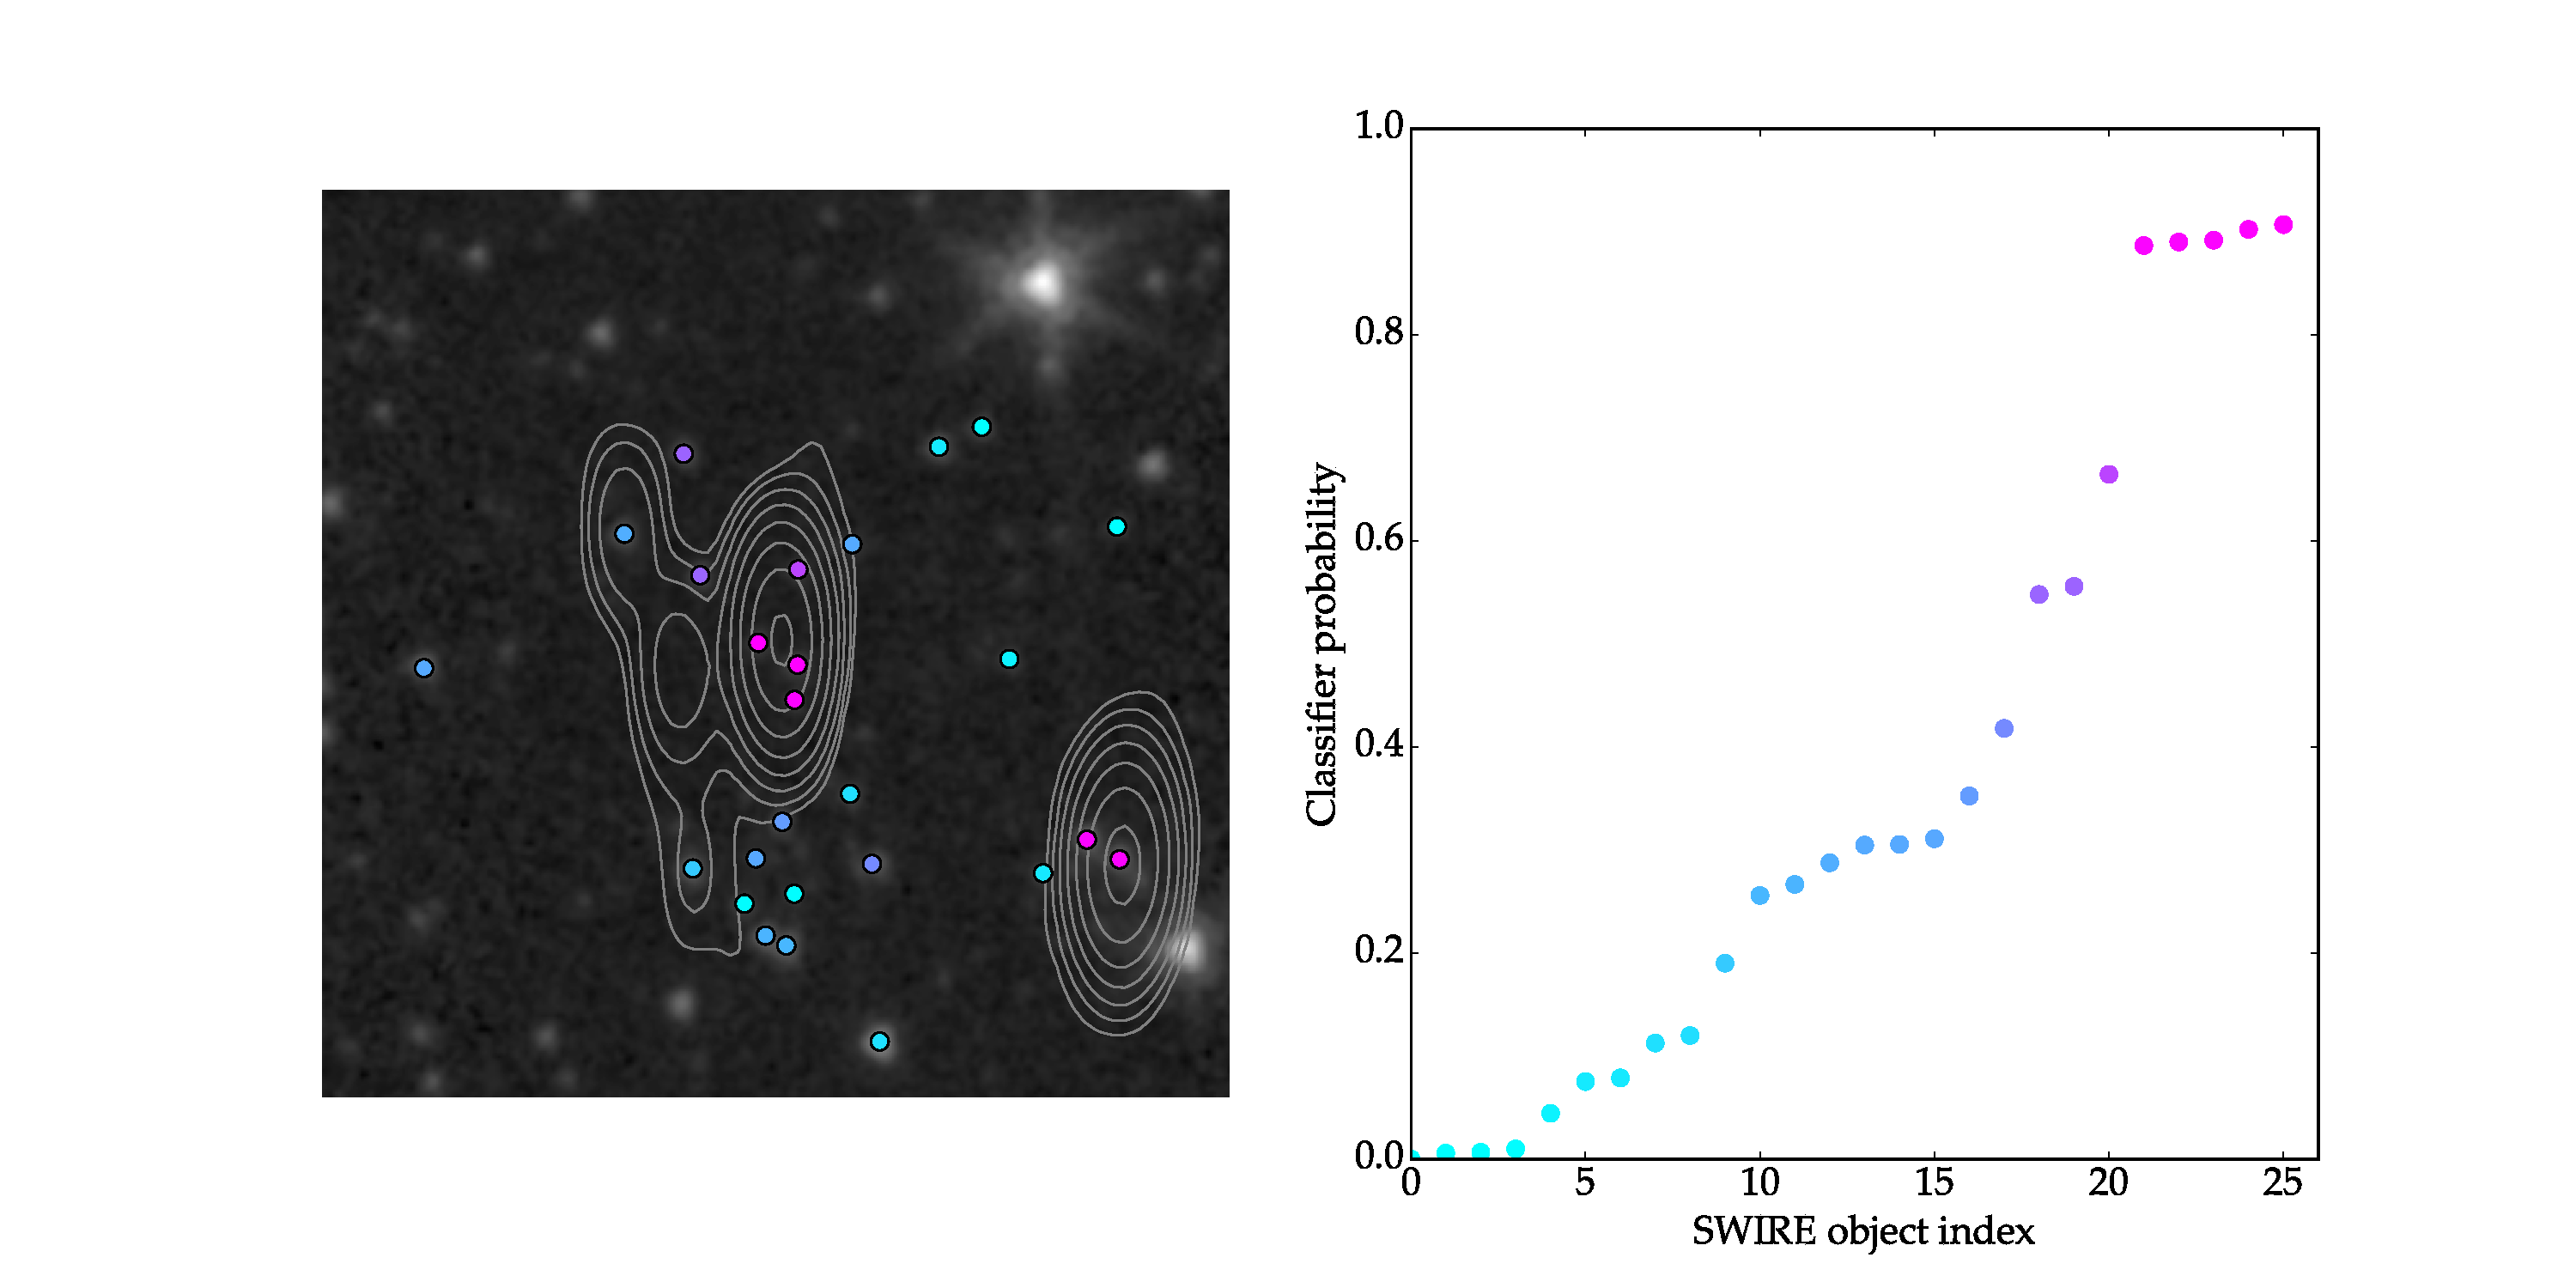
\includegraphics[width=\linewidth]{images/ARG0003r1r_lr.pdf}
      \caption{Logistic regression output for ARG0003r1r, consisting of two (possibly three) radio sources. This is hard to classify even for humans, and the difficulty is clear from the plot.}
      \label{fig:ARG0003r1r_lr}
    \end{figure}

  \newpage
  \section*{Appendix II}

    This appendix contains sample outputs from the random forest classifier. On the left of each figure is an ATLAS subject, with the infrared image from SWIRE in the background and intensity contours of the ATLAS radio image in the foreground. Candidate hosts are plotted on top of these images, coloured based on the predicted probability that they are the true host (where blue is least likely, and pink is most likely). On the right of each figure is a plot of each candidate's predicted probability with an arbitrary $x$ axis. The candidates have been sorted by increasing probability.

    \begin{figure}[!ht]
      \centering
      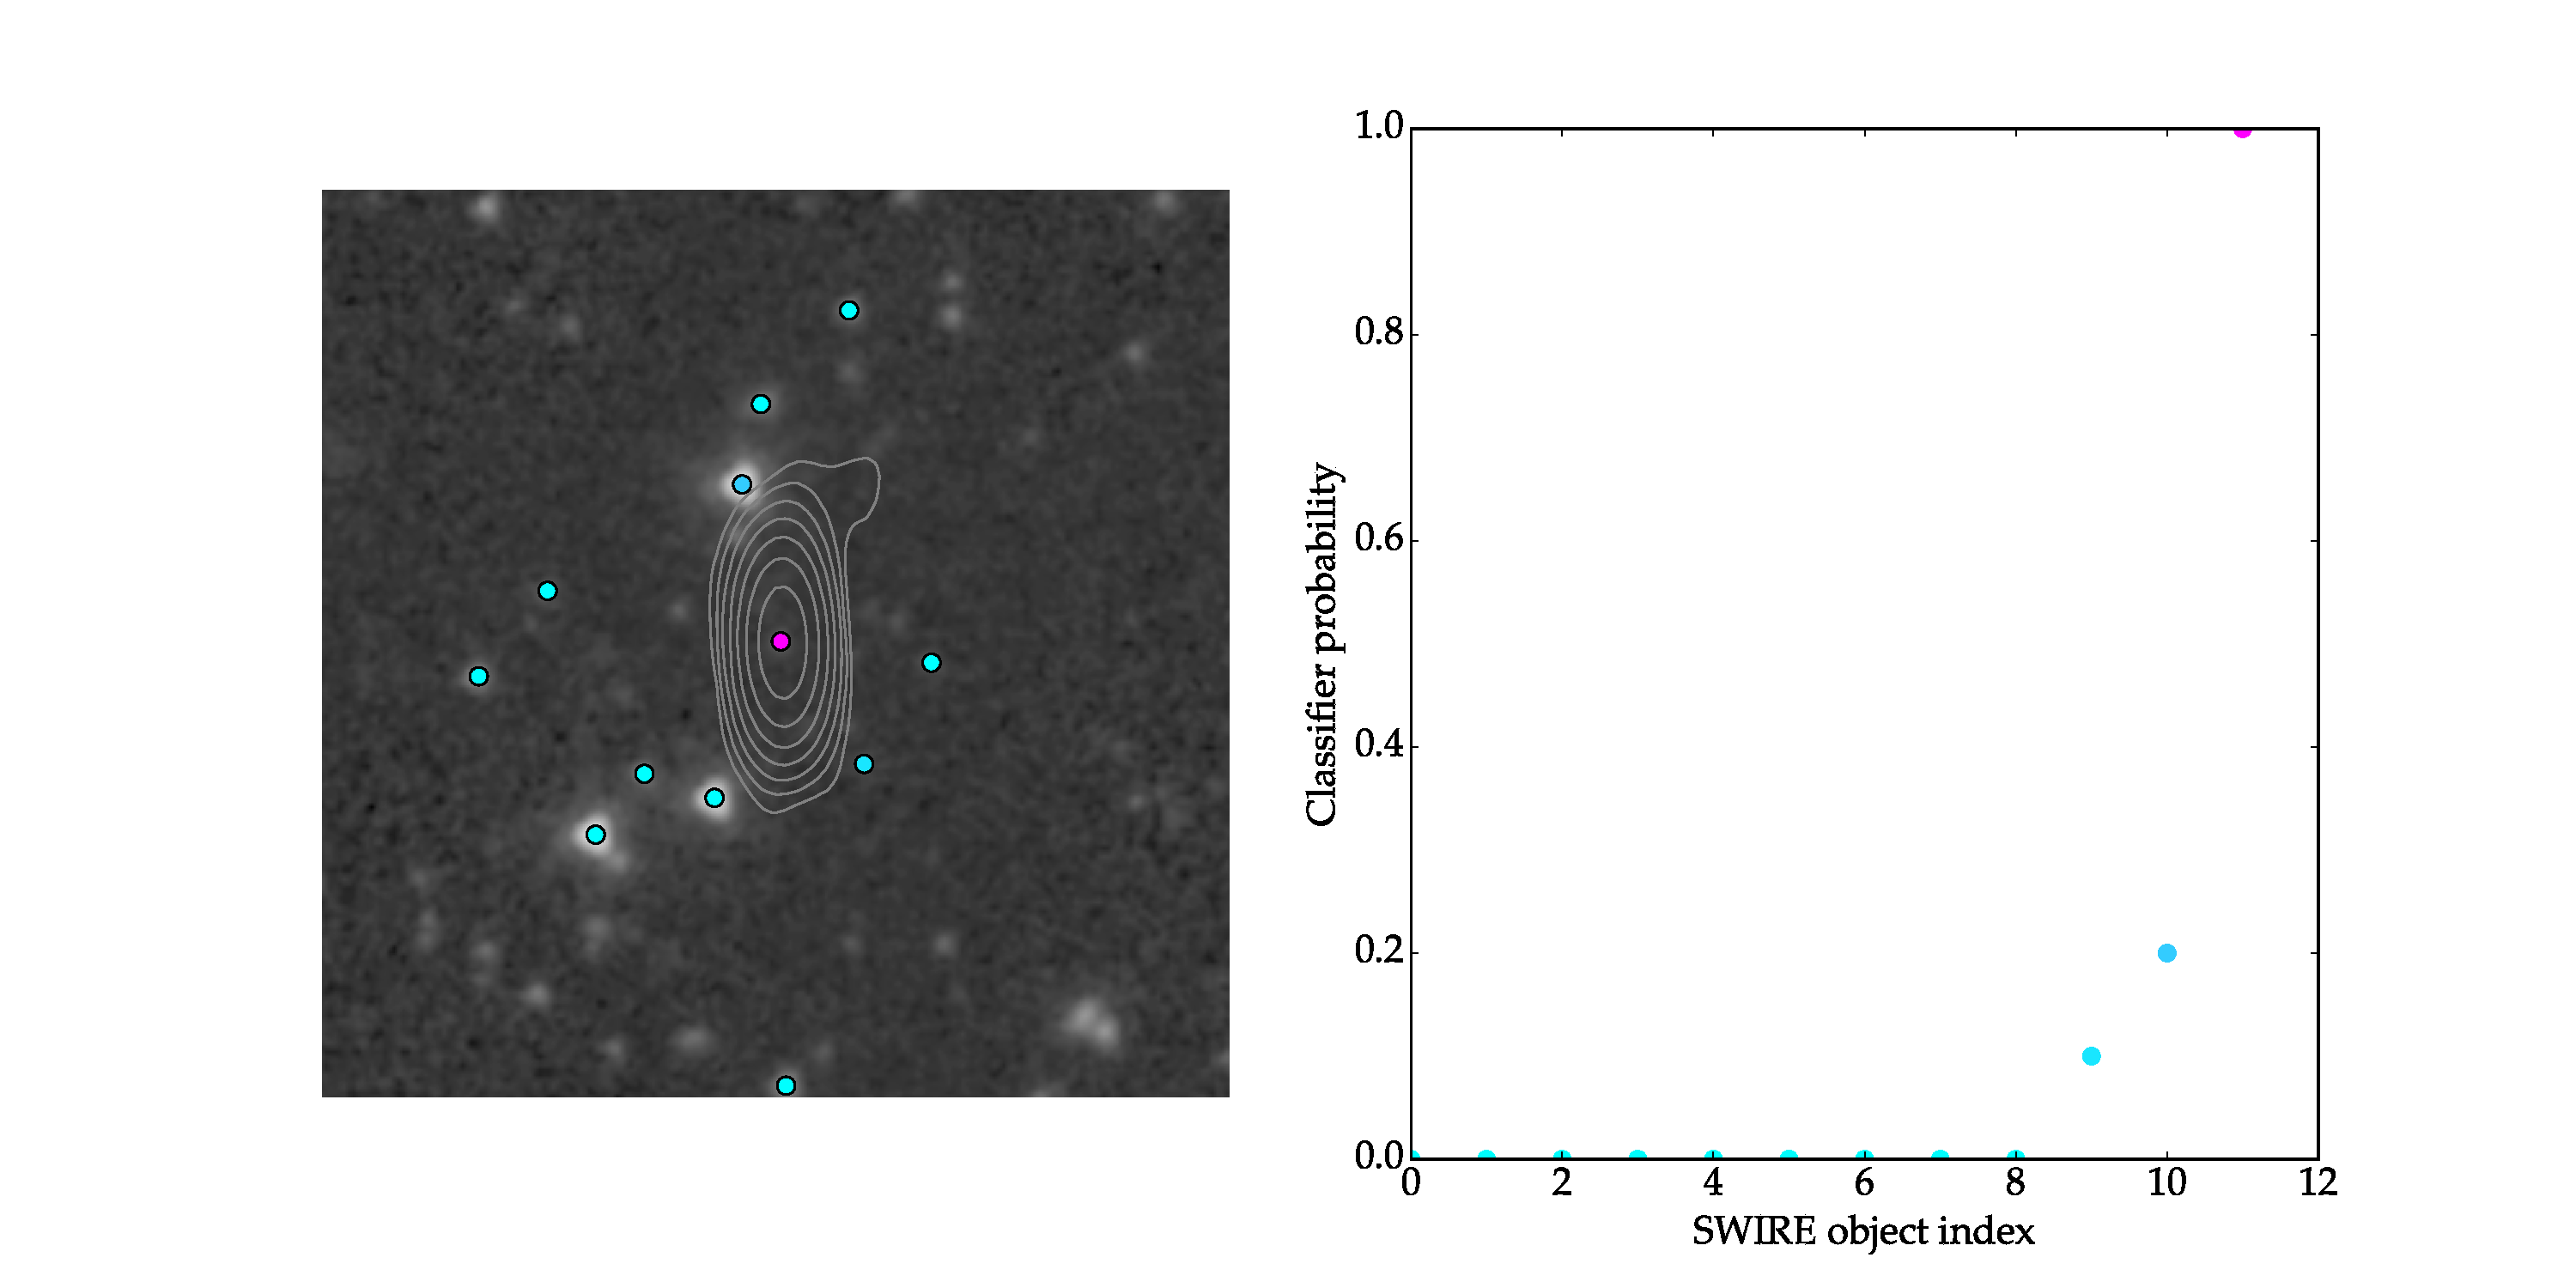
\includegraphics[width=\linewidth]{images/ARG0003r2o_rf.pdf}
      \caption{Random forests output for ARG0003r2o, an easy-to-classify compact source.}
      \label{fig:ARG0003r2o_rf}
    \end{figure}

    \begin{figure}[!ht]
      \centering
      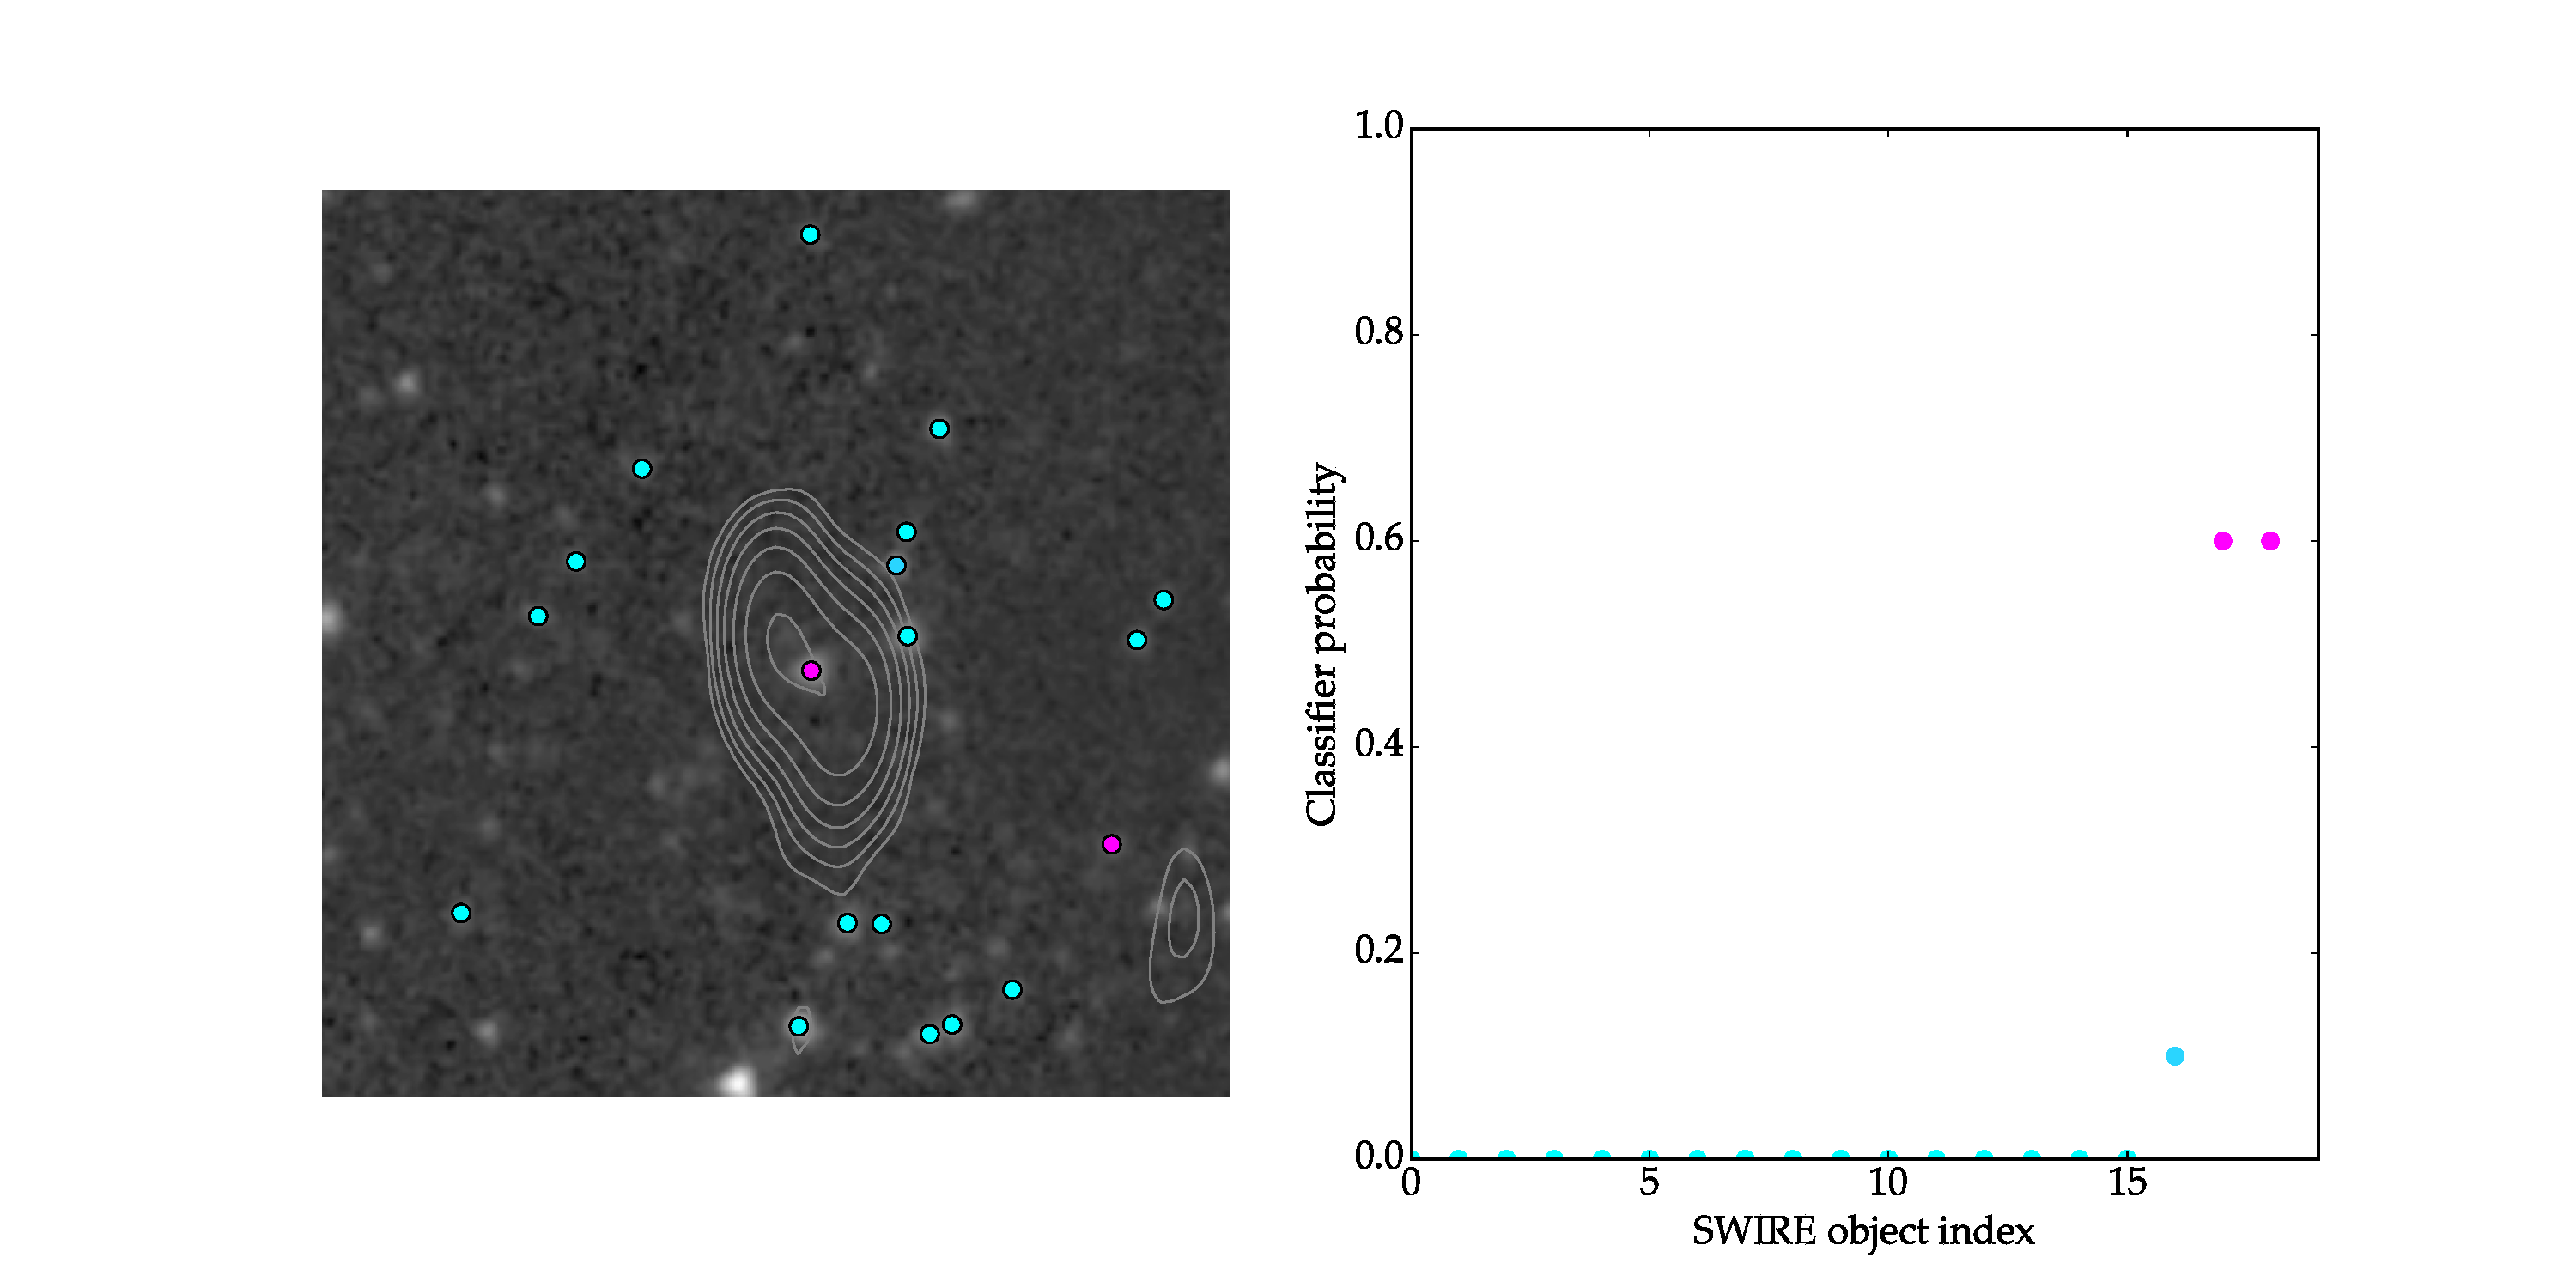
\includegraphics[width=\linewidth]{images/ARG0003r2w_rf.pdf}
      \caption{Random forests output for ARG0003r2w, a compact source. Logistic regression classifies this easily, but random forests finds two candidates with equal probability of being the true host.}
      \label{fig:ARG0003r2w_rf}
    \end{figure}

    \begin{figure}[!ht]
      \centering
      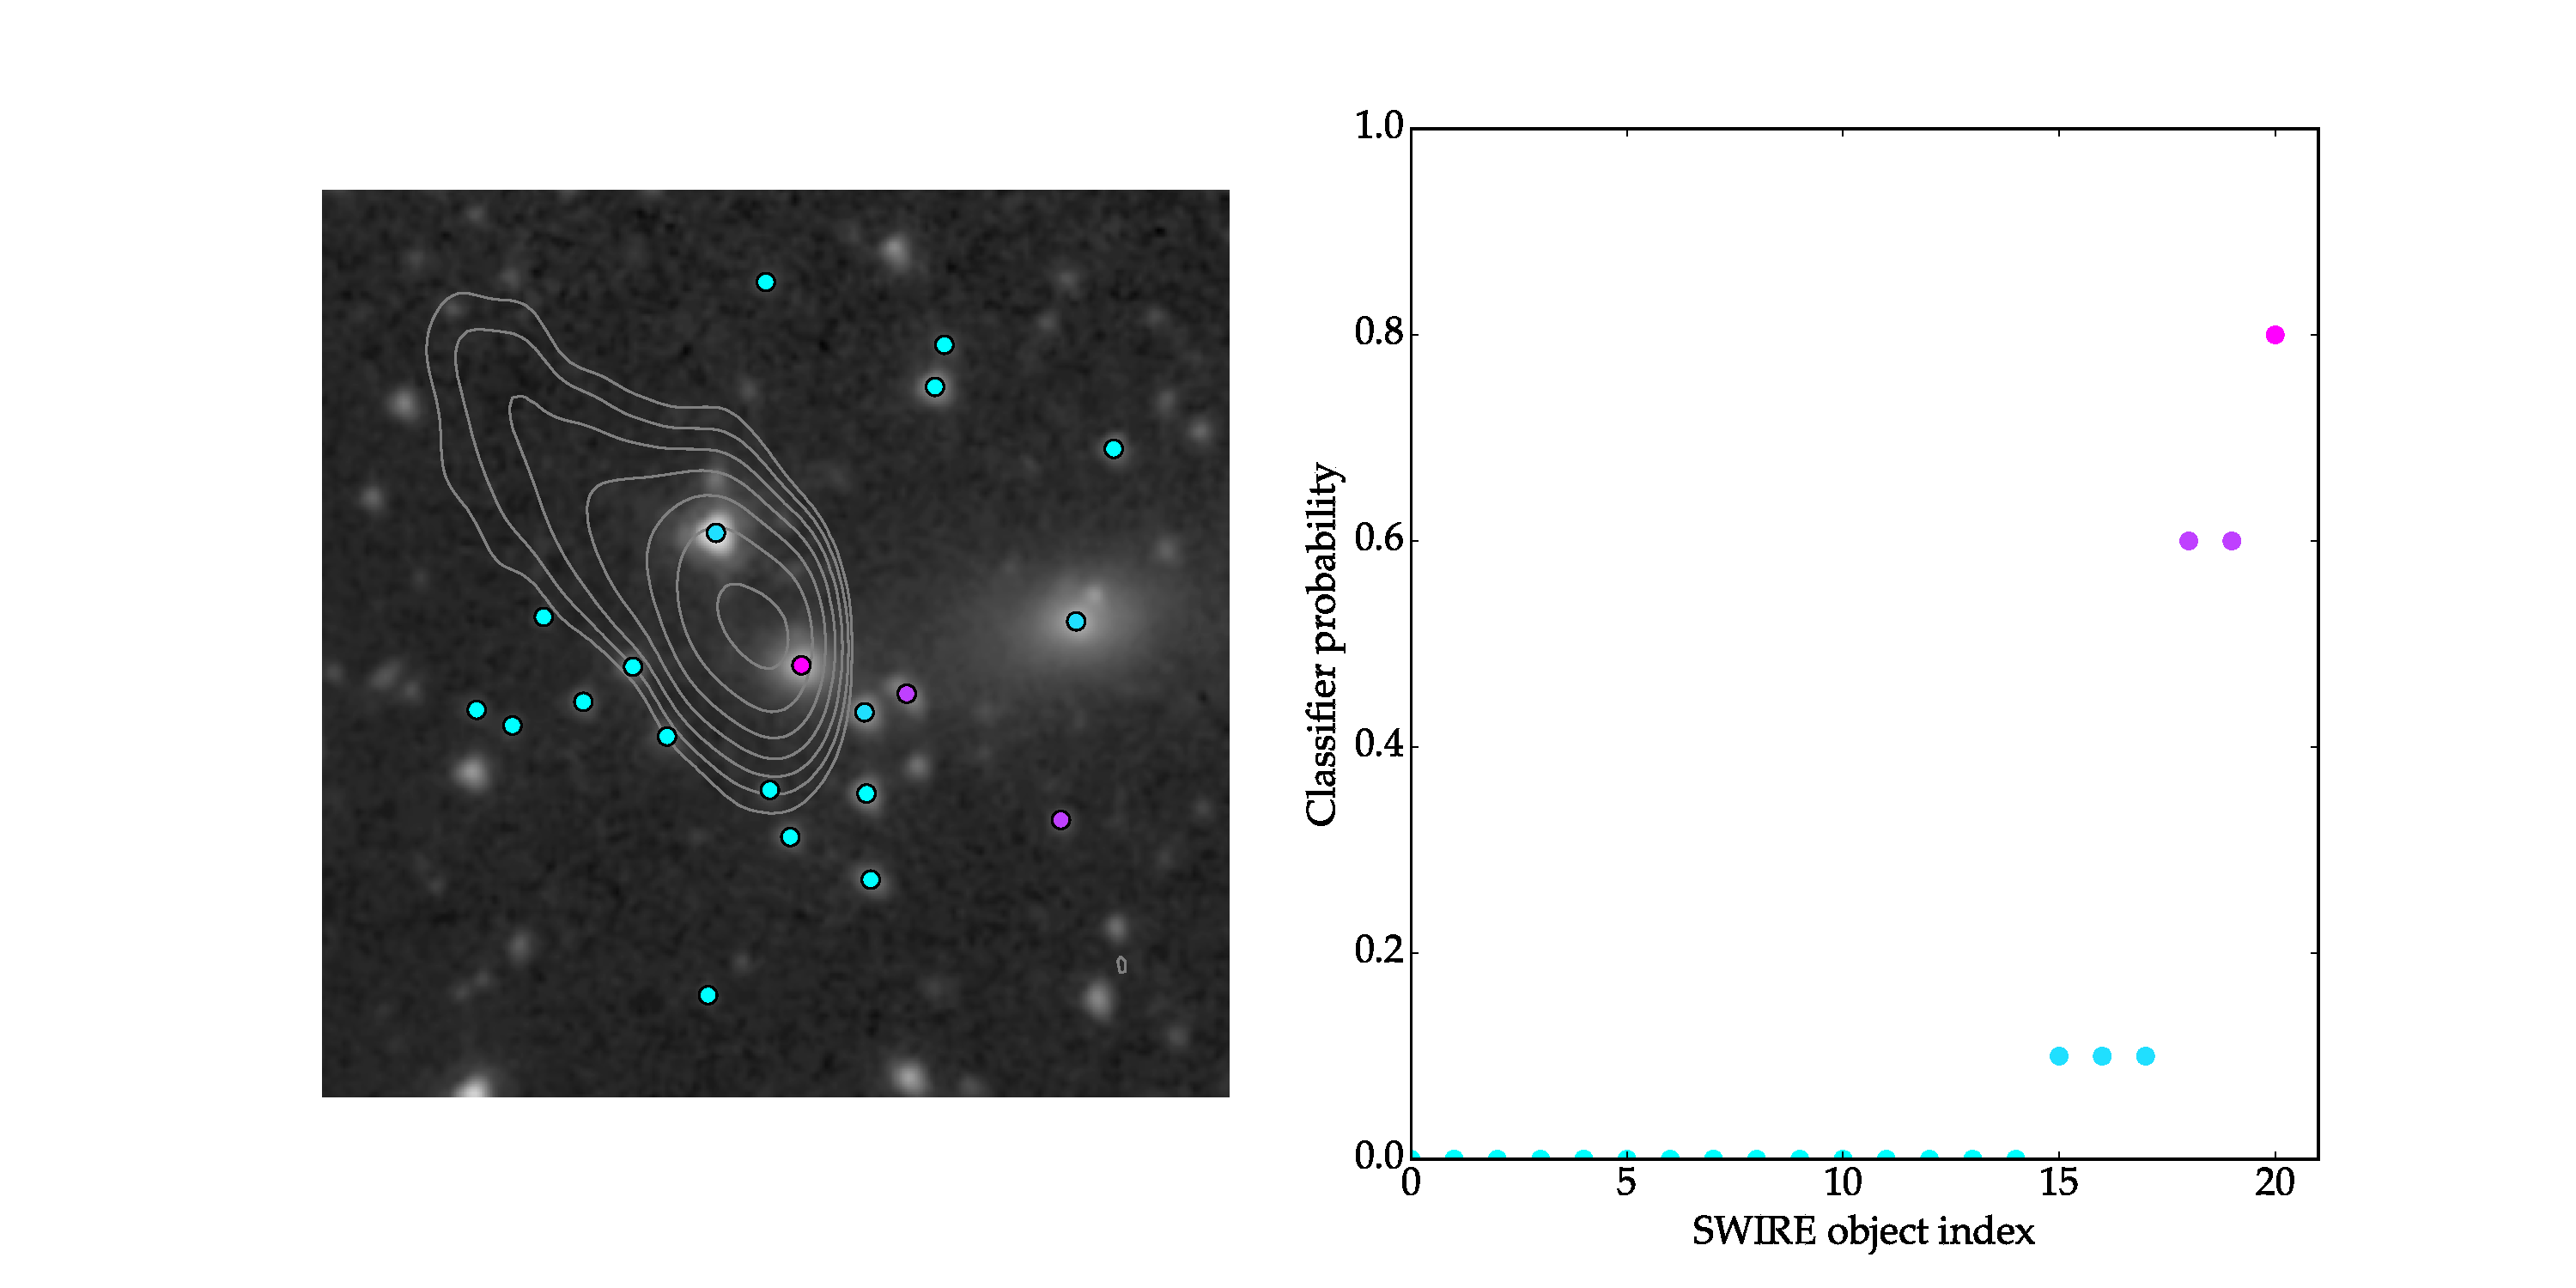
\includegraphics[width=\linewidth]{images/ARG0003r25_rf.pdf}
      \caption{Random forests output for ARG0003r25, a complex source.}
      \label{fig:ARG0003r25_rf}
    \end{figure}

    \begin{figure}[!ht]
      \centering
      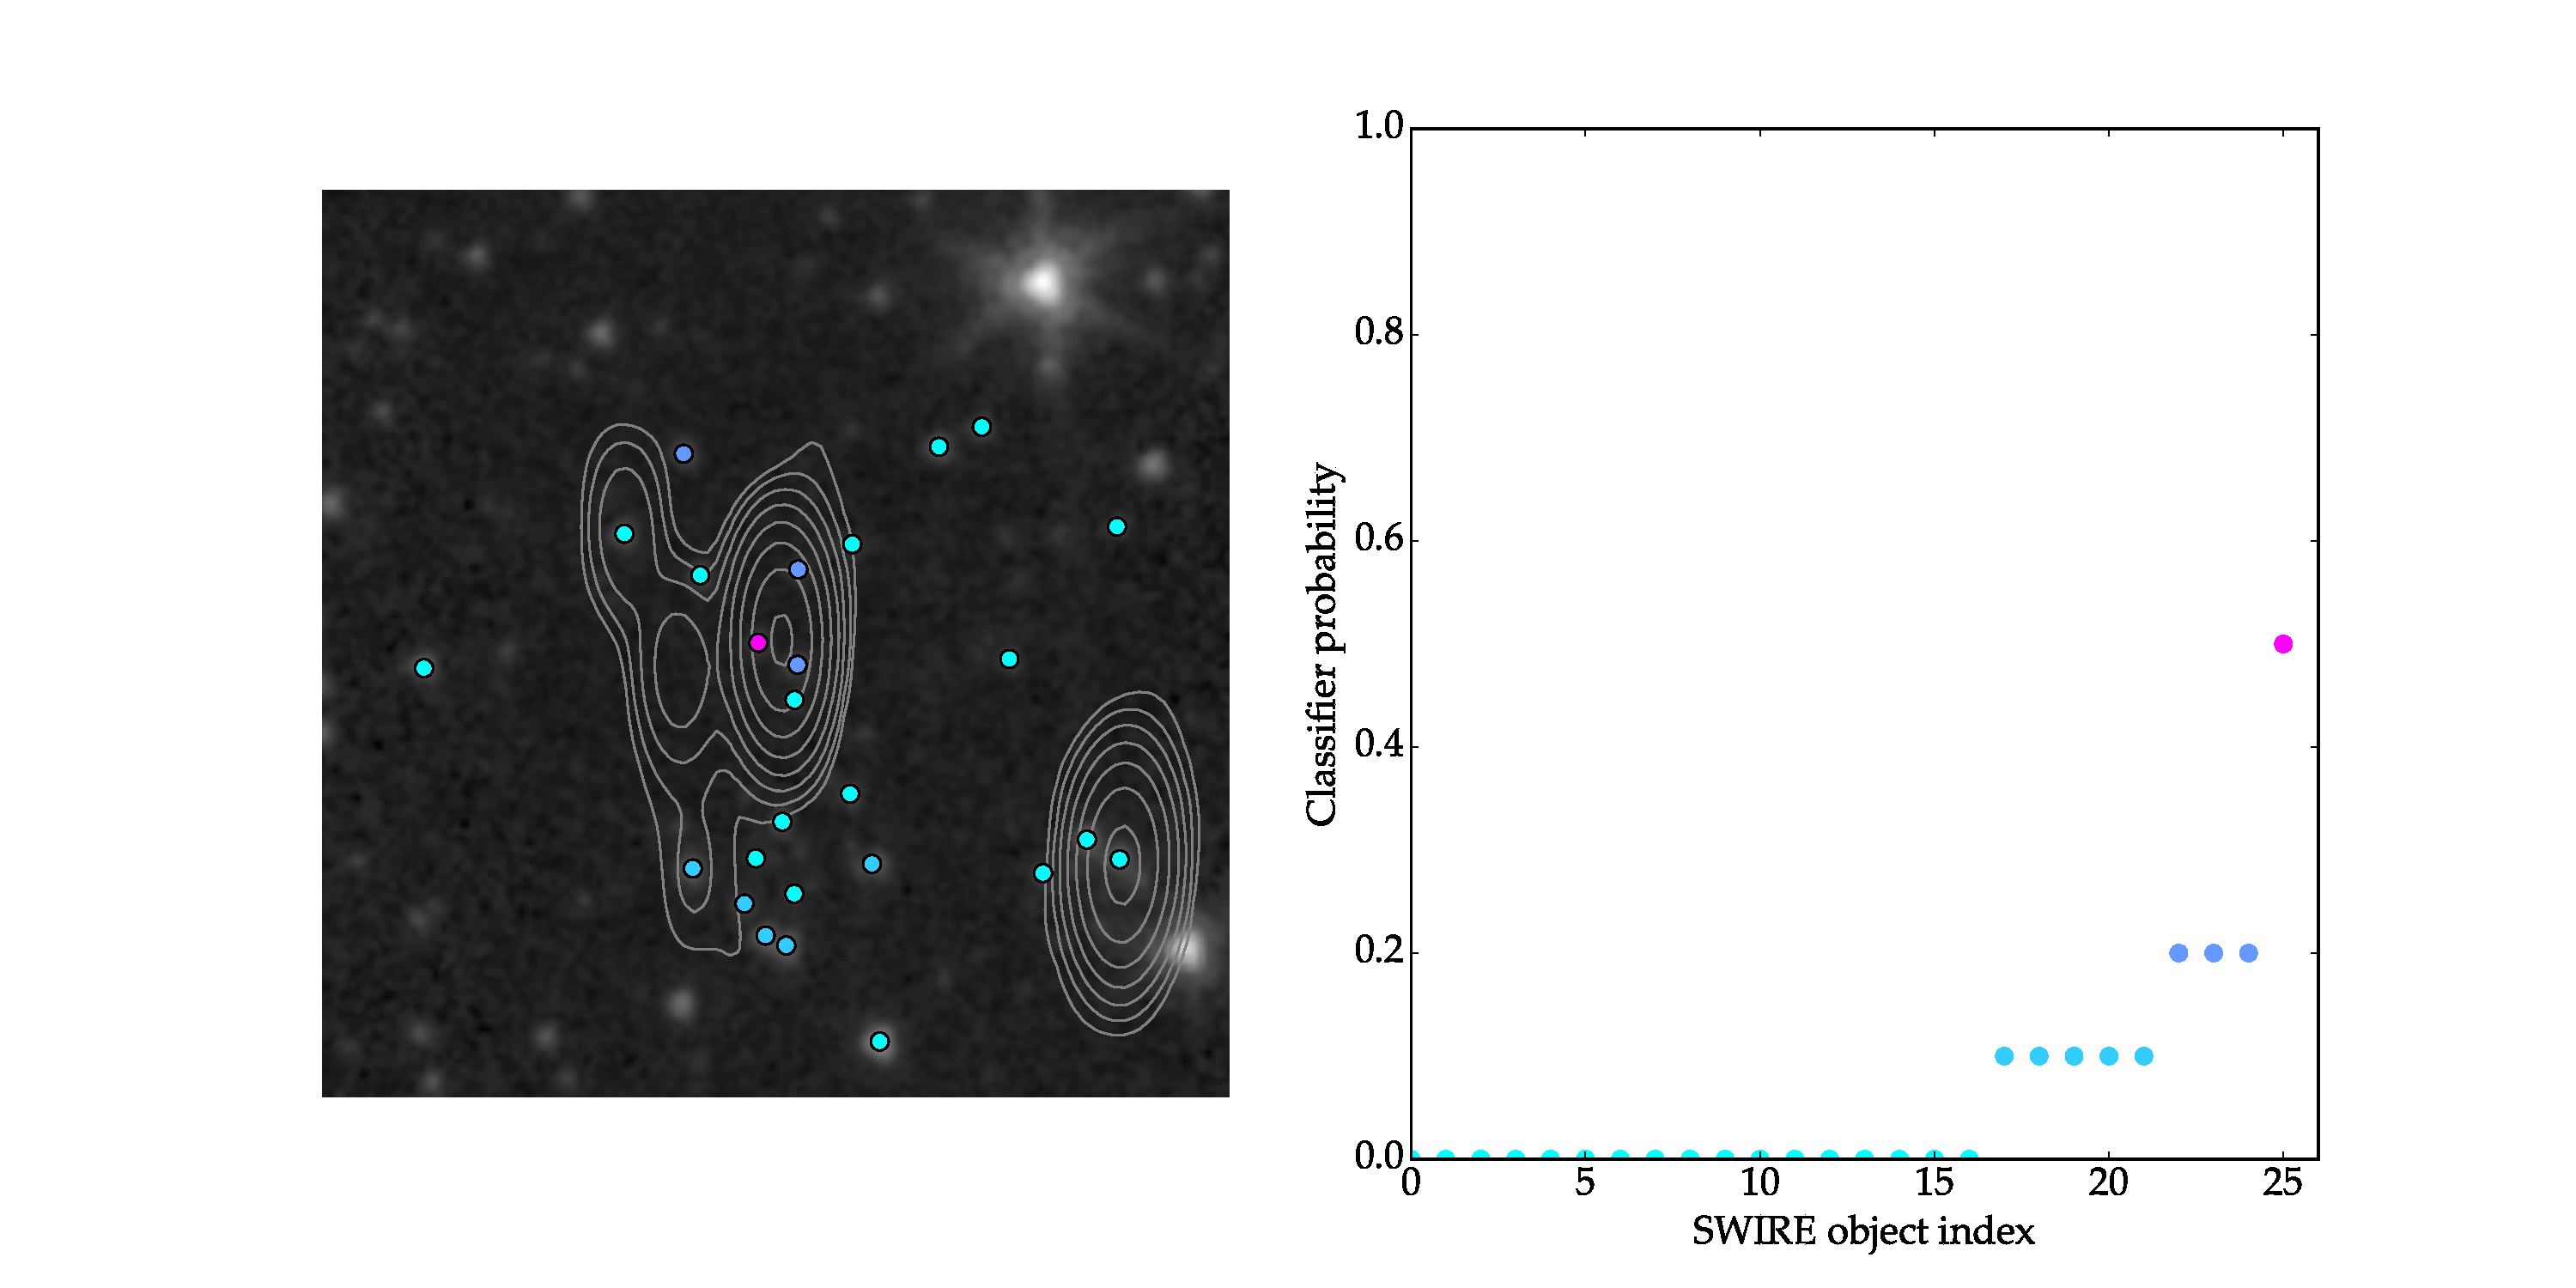
\includegraphics[width=\linewidth]{images/ARG0003r1r_rf.pdf}
      \caption{Random forests output for ARG0003r1r, consisting of two (possibly three) radio sources. Random forests does well on this subject despite it being quite complicated.}
      \label{fig:ARG0003r1r_rf}
    \end{figure}

\end{document}